\documentclass[a4paper,12pt]{article}

% ---------- Page layout ----------
\usepackage[a4paper,left=2cm,right=2cm,top=2cm,bottom=2cm]{geometry}
\usepackage{setspace}
\onehalfspacing

% ---------- Russian + normal fonts (pdfLaTeX) ----------
\usepackage[T2A]{fontenc}
\usepackage[utf8]{inputenc}
\usepackage[russian,english]{babel}

% ---------- Captions: "рис. N" ----------
\usepackage[labelsep=space]{caption} % <- важно: подпись будет "рис. 1"
\captionsetup[figure]{name=Рис. }
\usepackage{subcaption}

% ---------- Packages ----------
\usepackage{graphicx}
\usepackage{amsmath}
\usepackage{float}
\usepackage{siunitx}
\usepackage{booktabs}
\usepackage{afterpage}

\graphicspath{{.}}

\begin{document}

\tableofcontents
\clearpage 

\section{Введение: Физические основы и особенности диода Шоттки}

\textbf{Диод Шоттки} — это полупроводниковый прибор, выпрямительные свойства которого основаны на использовании перехода \textbf{металл--полупроводник}, а не $p\text{-}n$ перехода. Это принципиальное различие определяет ключевые эксплуатационные преимущества и область применения данных компонентов.

\subsection*{Основные отличия и преимущества}

В отличие от стандартных диодов, где носителям заряда необходимо преодолевать потенциальный барьер $p\text{-}n$ перехода, в диоде Шоттки процессы протекают иначе:

\begin{itemize}
    \item \textbf{Высокое быстродействие:} В диодах Шоттки (ДШ) отсутствуют процессы накопления и рассасывания неосновных носителей заряда, так как ток переносится только основными носителями — электронами. Это позволяет диоду переключаться почти мгновенно, что критично для работы в СВЧ-диапазоне и импульсных схемах.
    \item \textbf{Низкое прямое падение напряжения:} Напряжение включения у ДШ составляет примерно $0.2$--$0.4$~В, тогда как у обычных кремниевых диодов оно достигает $0.6$--$0.7$~В. Это значительно снижает потери энергии и тепловыделение.
    \item \textbf{Высокая плотность тока:} Конструктивные особенности позволяют пропускать значительные токи при малых габаритах элемента, что способствует эффективной микроминиатюризации.
\end{itemize}

\subsection*{Области применения}

Благодаря своим характеристикам, диоды Шоттки являются незаменимыми элементами в современной электронике:
\begin{enumerate}
    \item \textbf{Выпрямители:} Использование в высокочастотных блоках питания и солнечных батареях для минимизации потерь.
    \item \textbf{СВЧ-техника:} Применение в качестве детекторов и смесителей частоты (благодаря малой емкости перехода).
    \item \textbf{Логические схемы:} Использование для предотвращения насыщения транзисторов и увеличения скорости работы вычислительных комплексов.
\end{enumerate}

\newpage

\section{Цель работы}
\textbf{Цель работы:} Исследование физических принципов работы и экспериментальное определение основных параметров диода Шоттки на основе кремния $p$-типа.

\textbf{Задачи работы:}
\begin{enumerate}
    \item Овладение методикой изготовления контакта Шоттки (система кремний $p$-типа -- алюминий) и омического контакта (кремний $p$-типа -- золото).
    \item Экспериментальное снятие вольт-амперной характеристики (ВАХ) полученного диода Шоттки.
    \item Построение ВАХ в полулогарифмическом масштабе и проведение расчетного определения высоты потенциального барьера.
    \item Измерение контактной разности потенциалов на границе металл--полупроводник и проведение сравнительного анализа полученного значения с высотой барьера Шоттки.
    \item Расчет емкости диода Шоттки и проведение сравнительного анализа с характеристиками стандартного диода на основе полупроводникового $p\text{-}n$ перехода.
\end{enumerate}

% ===== ДОБАВЛЕНО (из методички): объект/оборудование =====
\section{Оборудование}
Измерения проводятся на стенде, включающем микроскоп, два микроманипулятора с зондами,
платформу с вакуумной фиксацией образца, АЦП и ЭВМ со специализированным программным
обеспечением для автоматического съёма ВАХ и ВФХ. Образец - кремниевая пластина (КДБ10) n-типа с изолирующим слоем SiO2, содержащая напыленные (Шоттки) и вплав-ленные (омические) контакты Al, а также контакты Au.

\section{Теоретическая часть}

Диод Шоттки представляет собой выпрямитель тока, основанный на нелинейном характере электрической проводимости контакта металла с полупроводником. В отличие от других видов электронных выпрямителей (электровакуумные диоды или диоды на основе полупроводниковых p-n-переходов), диоды Шоттки характеризуются:
\begin{itemize}
    \item высокой плотностью тока;
    \item повышенным быстродействием;
    \item возможностями микроминиатюризации.
\end{itemize}

Диоды Шоттки широко используются в технике СВЧ в качестве детекторов, смесителей частоты, умножителей, переключателей и других типов вентильных элементов.

\subsection{Энергетические диаграммы металла и полупроводника}

Механизм работы диода Шоттки обычно рассматривают с помощью энергетической диаграммы. На энергетических диаграммах принято откладывать по оси ординат полную энергию электрона, а по оси абсцисс --- пространственную координату.

Энергию находящегося на бесконечности и покоящегося электрона принимают равной нулю. Энергетическая диаграмма свободного пространства состоит из одной горизонтальной прямой, проходящей через 0 оси ординат.

Энергетическая диаграмма металла имеет вид потенциальной ямы (рис. 1а). Энергия электронов, находящихся в потенциальной яме, может принимать лишь дискретные значения. Вероятность заполнения $f$ электронами уровня с энергией $E$ описывается функцией Ферми-Дирака:

\begin{equation}
f(E) = \frac{1}{\exp\left(\frac{E - E_F}{kT}\right) + 1},
\end{equation}

где $T$ --- температура, $E_F$ --- энергия Ферми, $k$ --- постоянная Больцмана.

\begin{figure}[h]
\centering
% Placeholder for Figure 1: Energy diagrams
% This figure should show four energy diagrams:
% (a) Metal - potential well with Fermi level
% (b) Dielectric/intrinsic semiconductor - showing conduction band, valence band, and band gap
% (c) n-type semiconductor - with donor levels near conduction band
% (d) p-type semiconductor - with acceptor levels near valence band
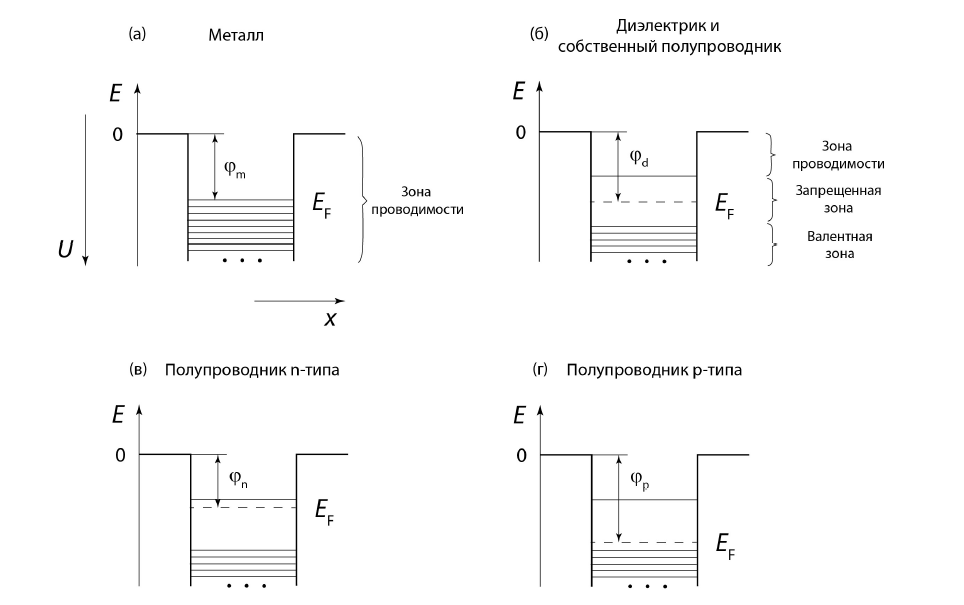
\includegraphics[width=0.9\textwidth]{image.png}
\caption{Энергетические диаграммы: (а) металла, (б) диэлектрика и собственного полупроводника, (в) полупроводника n-типа, (г) полупроводника p-типа}
\label{fig:energy_diagrams}
\end{figure}

Минимальная работа, необходимая для удаления электрона из металла на бесконечность, называется работой выхода и равна $\varphi_m = -E_F$.

Энергетическая диаграмма диэлектрика (или собственного полупроводника) показана на рис. 1б. Она представляет собой потенциальную яму, в которой расположены три зоны: зона проводимости (ЗП), запрещенная зона (ЗЗ) и валентная зона (ВЗ).

Энергетические диаграммы примесных полупроводников представлены на рис. 1в и 1г:
\begin{itemize}
    \item У донорной примеси энергетические уровни располагаются в запрещенной зоне немного ниже дна зоны проводимости (n-тип проводимости);
    \item Акцепторная примесь имеет уровни немного выше потолка валентной зоны (p-тип проводимости).
\end{itemize}

\subsection{Потенциальный барьер на границе металл-полупроводник}

Электрические характеристики контакта металл-полупроводник существенно зависят от соотношения между работами выхода электронов из металла $\varphi_m$ и полупроводника $\varphi_s$, а также от типа проводимости последнего.

Рассмотрим контакт между металлом и донорным полупроводником с $\varphi_n < \varphi_m$. Энергетические диаграммы незаряженных и не находящихся в механическом и электрическом контакте металла и полупроводника показаны на рис. 2а.

При обеспечении электрического контакта электроны из зоны проводимости полупроводника переходят в металл, заряжая его отрицательно. При этом между полупроводником и металлом возникает контактная разность потенциалов:

\begin{equation}
U_0 = \frac{\varphi_m - \varphi_n}{e},
\end{equation}

а в пространстве между ними возникает электрическое поле $\varepsilon = \frac{U_0}{d}$, где $d$ --- расстояние между металлом и полупроводником.

\begin{figure}[h]
\centering
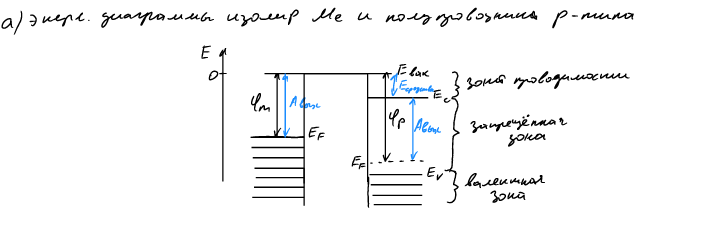
\includegraphics[width=0.9\textwidth]{pp1.png}
\label{fig:barrier_formation}
\end{figure}

\begin{figure}[h]
\centering
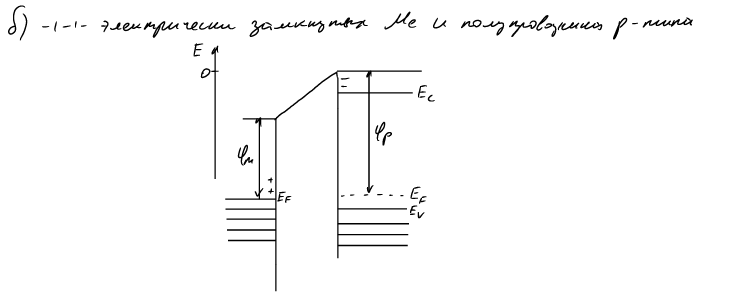
\includegraphics[width=0.9\textwidth]{pp2.png}
\label{fig:barrier_formation}
\end{figure}

\begin{figure}[h]
\centering
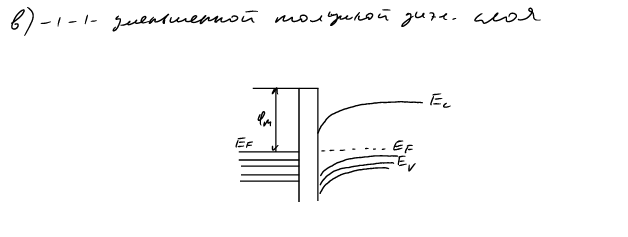
\includegraphics[width=0.9\textwidth]{pp3.png}
\label{fig:barrier_formation}
\end{figure}

\begin{figure}[h]
\centering
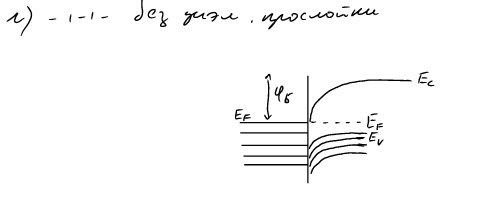
\includegraphics[width=0.9\textwidth]{pp5.png}
\label{fig:barrier_formation}
\end{figure}

На энергетической диаграмме (рис. 2в) можно различить два энергетических барьера:
\begin{itemize}
    \item узкий барьер с высотой над уровнем Ферми $\varphi_m$ (толщина $\sim 10$ Å);
    \item широкий барьер с высотой $\varphi_b = (\varphi_m - \varphi_n) = eU_0$.
\end{itemize}

Узкий барьер не препятствует обмену электронами за счет эффекта квантовомеханического туннелирования. Электрические характеристики контакта определяет широкий барьер высотой $\varphi_b = eU_0$, называемый \textbf{барьером Шоттки}.

\subsection{Вольт-амперная характеристика выпрямляющего контакта}

Барьер Шоттки затрудняет обмен носителями заряда между металлом и полупроводником. Ток термоэлектронной эмиссии можно оценить по формуле:

\begin{equation}
I_0 = S A_0 T^2 e^{-\frac{\varphi_b}{kT}},
\end{equation}

где 
\begin{equation}
A_0 = \frac{4\pi e m k^2}{h^3} \approx 120 \text{ А}/(\text{см}^2\cdot\text{К}^2),
\end{equation}

$S$ --- площадь контакта, $m$ --- масса электрона, $h$ --- постоянная Планка.

Полный ток через контакт складывается из токов термоэлектронной эмиссии, текущих из металла в полупроводник и из полупроводника в металл.

При подаче на полупроводник отрицательного напряжения $-U$ (прямое смещение) энергетическая диаграмма показана на рис. 3б. Высота потенциального барьера для тока из полупроводника в металл уменьшается на величину $eU$.

\begin{figure}[h]
\centering
% Placeholder for Figure 3: Energy diagrams under bias
% This figure should show three energy diagrams:
% (a) Zero bias U=0 - symmetric barriers
% (b) Reverse bias U<0 - increased barrier for semiconductor to metal
% (c) Forward bias U>0 - decreased barrier for semiconductor to metal
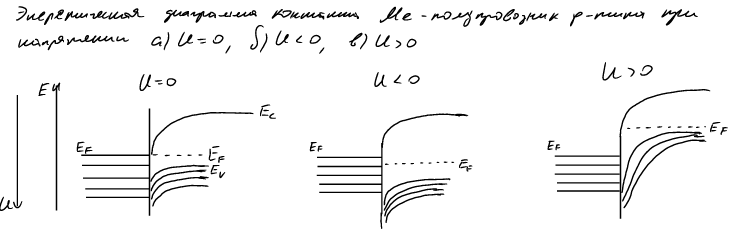
\includegraphics[width=0.9\textwidth]{pp6.png}
\caption{Энергетическая диаграмма контакта металл-полупроводник при внешнем напряжении: (а) U=0, (б) U<0, (в) U>0}
\label{fig:bias_diagrams}
\end{figure}

Суммарный ток через контакт равен:

\begin{equation}
I = S A_0 T^2 e^{-\frac{\varphi_b - eU}{kT}} - S A_0 T^2 e^{-\frac{\varphi_b}{kT}} = I_0 \left(e^{\frac{eU}{kT}} - 1\right).
\end{equation}

При подаче положительного напряжения (обратное смещение, рис. 3в) общий ток через контакт описывается той же формулой (5).

\begin{figure}[h]
\centering
% Placeholder for Figure 4: I-V characteristic of Schottky diode
% This figure should show the typical I-V curve of a Schottky diode:
% - Exponential growth in forward bias region
% - Small saturation current in reverse bias region
% - Mark the turn-on voltage and breakdown region if applicable
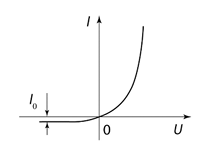
\includegraphics[width=0.7\textwidth]{p1.png}
\caption{Вольт-амперная характеристика диода Шоттки}
\label{fig:iv_characteristic}
\end{figure}

\subsection{Омический контакт}

Рассмотрим контакт между металлом и полупроводником с $\varphi_m < \varphi_n$ (рис. 5). Электрическое поле в полупроводнике подтягивает электроны зоны проводимости к области контакта, в результате чего образуется обогащенный электронами контактный слой. Потенциальный барьер отсутствует, и контакт является омическим.

\begin{figure}[h]
\centering
% Placeholder for Figure 5: Ohmic contact energy diagram
% This figure should show:
% - Metal and n-type semiconductor with φm < φn
% - Band bending that accumulates electrons at the interface
% - No barrier for electron flow in either direction
% - Linear (ohmic) behavior indicated
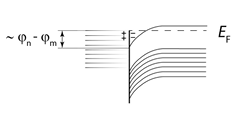
\includegraphics[width=0.7\textwidth]{p2.png}
\caption{Энергетическая диаграмма контакта металл-полупроводник с $\varphi_m < \varphi_n$ (омический контакт)}
\label{fig:ohmic_contact}
\end{figure}

Вольт-амперная характеристика такой структуры описывается законом Ома и является линейной.

Сопротивление растекания $R_r$ круглого металлического контакта радиуса $r$, расположенного на поверхности пластины полупроводника толщиной $d$, определяется выражением:

\begin{equation}
R_r = \frac{\rho}{2\pi r} \arctan\left(\frac{2d}{r}\right),
\end{equation}

где $\rho$ --- удельное сопротивление полупроводника.

\subsection{Сравнение теории с опытом}

Для сравнения с теорией строят прямую ветвь вольт-амперной характеристики в полулогарифмическом масштабе (рис. 6).

\begin{figure}[h]
\centering
% Placeholder for Figure 6: Semi-log I-V plot
% This figure should show:
% - Semi-logarithmic plot (log I vs U)
% - Linear region in forward bias
% - Indication of how to extract ideality factor from slope
% - Extrapolation to U=0 to find I0
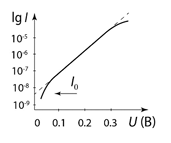
\includegraphics[width=0.7\textwidth]{p3.png}
\caption{Аппроксимация вольт-амперной характеристики в полулогарифмическом масштабе}
\label{fig:semilog_plot}
\end{figure}

Прямолинейный участок аппроксимируется выражением:

\begin{equation}
\ln I = \ln(S A_0 T^2) - \frac{\varphi_b}{kT} + \frac{e}{\gamma kT} U,
\end{equation}

где $\gamma$ --- коэффициент идеальности, учитывающий возможные отклонения от диодной теории.

Коэффициент идеальности определяется из тангенса угла наклона характеристики:

\begin{equation}
\gamma = \frac{e}{kT} \left(\frac{d \ln I}{dU}\right)^{-1}.
\end{equation}

Значения $\gamma$ обычно лежат в пределах $1-2$.

Линейно экстраполируя характеристику к нулевому напряжению, находят $I_0$ и вычисляют высоту барьера:

\begin{equation}
\varphi_b = kT \ln\left(\frac{S A_0 T^2}{I_0}\right).
\end{equation}

\subsection{Роль поверхностных электронных состояний}

Поверхностные электронные состояния возникают на поверхности полупроводника в результате:
\begin{itemize}
    \item обрыва кристаллической решетки;
    \item дефектов поверхности;
    \item адсорбции чужеродных атомов.
\end{itemize}

\begin{figure}[h]
\centering
% Placeholder for Figure 7: Surface states in silicon
% This figure should show:
% (a) n-type silicon surface with surface states in band gap
% (b) p-type silicon surface with surface states
% - Show band bending due to surface states
% - Indicate Fermi level pinning effect
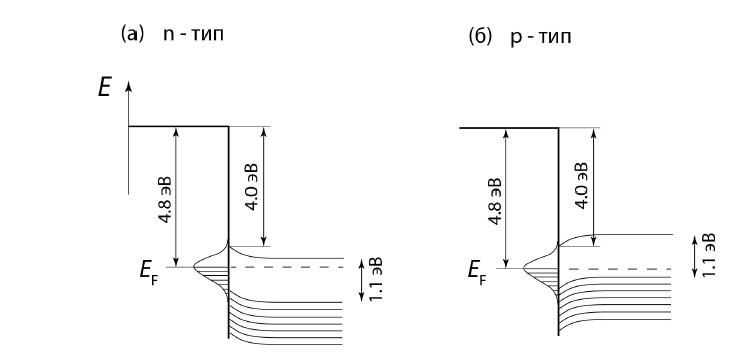
\includegraphics[width=0.9\textwidth]{image7.png}
\caption{Энергетические диаграммы поверхности кремния: (а) n-типа, (б) p-типа}
\label{fig:surface_states}
\end{figure}

На идеально чистой поверхности кремния имеется около $10^{15}$ см$^{-2}$ незаполненных ковалентных связей. За счет поверхностных состояний работа выхода электронов из кремния практически не зависит от типа проводимости (рис. 7).

\subsection{Промежуточный слой окисла}

В процессе изготовления или старения контакта между металлом и полупроводником может вырасти тонкий слой окисла:
\begin{itemize}
    \item При толщине до $10$ Å --- не оказывает влияния на электрические свойства;
    \item При толщине $10-100$ Å --- снижает плотность поверхностных состояний за счет туннельного эффекта;
    \item При толщине более $100$ Å --- обмен носителями происходит только через зону проводимости окисла.
\end{itemize}

\begin{figure}[h]
\centering
% Placeholder for Figure 8: Metal-insulator-semiconductor structure
% This figure should show:
% - Al-SiO2-Si(n-type) structure energy diagram
% - Metal, thin oxide layer, and semiconductor
% - Band bending in semiconductor
% - Tunneling through thin oxide layer indicated
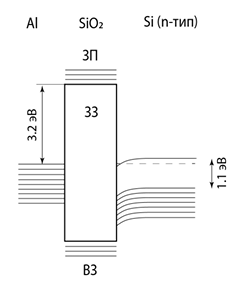
\includegraphics[width=0.5\textwidth]{p4.png}
\caption{Энергетическая диаграмма структуры металл-диэлектрик-полупроводник}
\label{fig:mis_structure}
\end{figure}

\subsection{Технология изготовления диода Шоттки}

\begin{figure}[h]
\centering
% Placeholder for Figure 9: Schottky diode structure
% This figure should show a cross-sectional view of a Schottky diode:
% - Top metal contact (e.g., Pt or Al)
% - n-type silicon substrate
% - p-type guard ring around the contact
% - Back ohmic contact
% - Indicate PtSi formation region if applicable
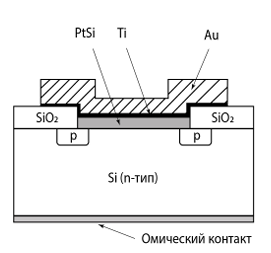
\includegraphics[width=0.8\textwidth]{p5.png}
\caption{Пример структуры диода Шоттки}
\label{fig:diode_structure}
\end{figure}

Промышленная технология изготовления диодов Шоттки весьма сложна. Для ослабления краевых эффектов края контакта окружают полупроводником противоположного типа проводимости.

\subsection{Основные формулы для расчетов}

Для обработки экспериментальных данных используются следующие формулы:

\begin{figure}[h]
\centering
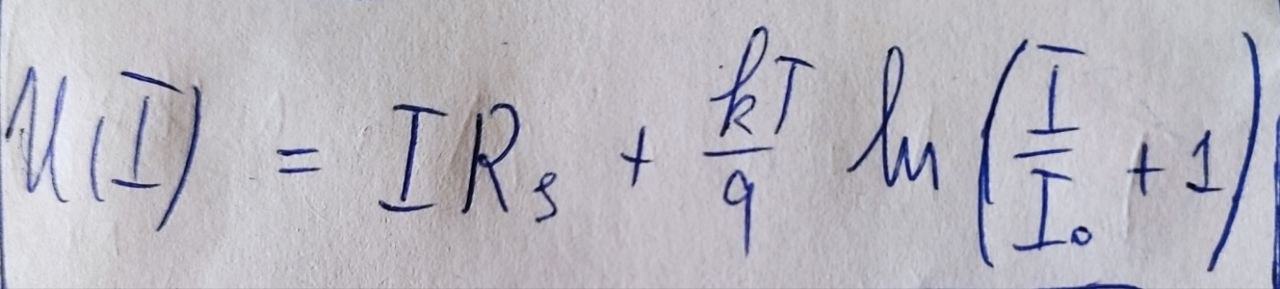
\includegraphics[width=0.9\textwidth]{pp7.jpg}
\label{fig:barrier_formation}
\end{figure}

\begin{figure}[h]
\centering
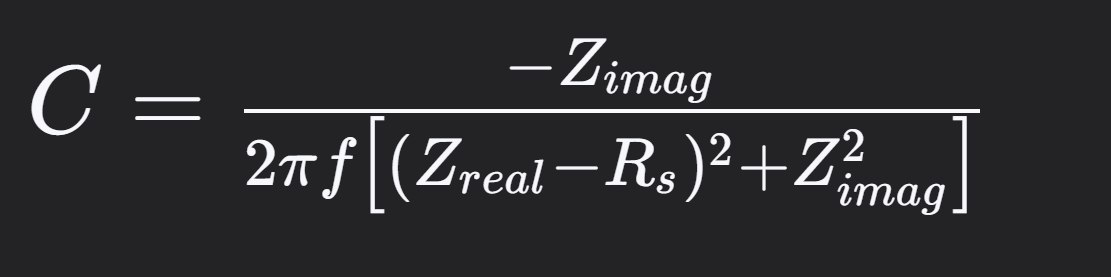
\includegraphics[width=0.9\textwidth]{pp8.jpg}
\label{fig:barrier_formation}
\end{figure}

\section{Ход работы}
\subsection{Измерение параметров омического контакта Al на Si}
\subsubsection*{Измерение ВАХ алюминиевой рамки}
Установим зонды на алюминиевой рамке. Сначала измерим ВАХ на одном расстроянии и определим полное сопротивление по графику, после чего, увеличив расстояние, найдем новое сопротивление. Из полученных данных найдем погонную плотность рамки и внутреннее сопротивление схемы. 
\[R_1=5,65 \text{ Ом}, L_1 = 523, 4 \text{ мкм}, R_2=    6,59 \text{ Ом}, L_1 = 4043,0 \text{ мкм}\]
\[
\lambda=\frac{R_2-R_1}{L_2-L_1}
=254\text{ Ом/м}
\]
\[
R_\text{внутреннее} = R_2 - \lambda \cdot L_2 = 5,5\text{ Ом}
\]
\begin{figure}[H]
    \centering
    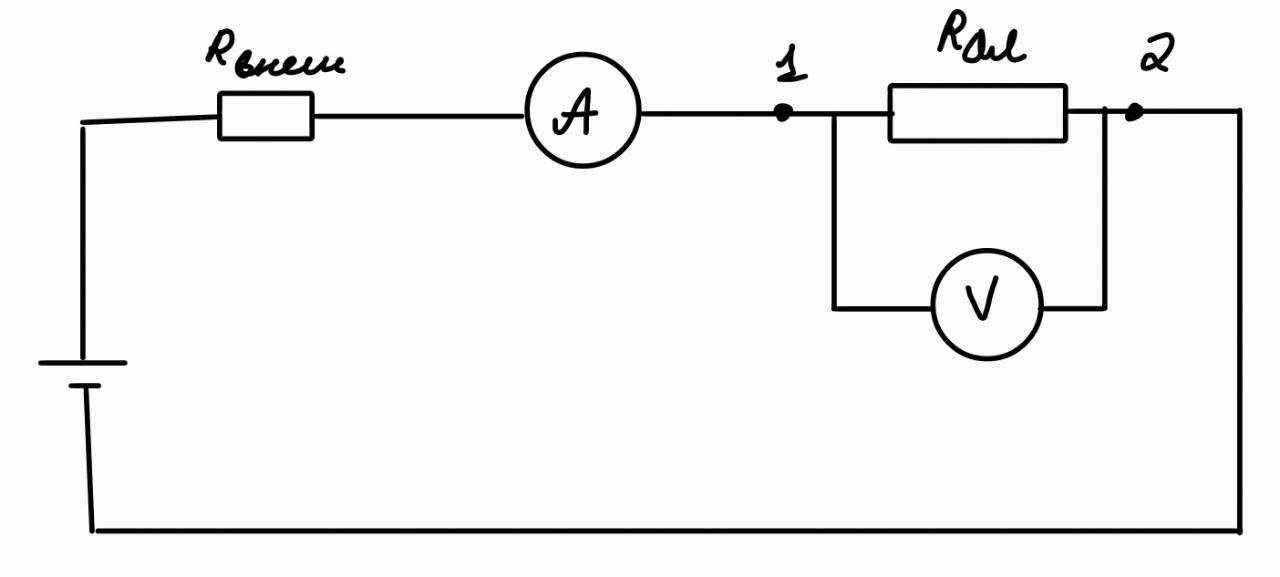
\includegraphics[width=0.5\linewidth]{image8.png}
    \caption{Электрическая схема измерения ВАХ алюминиевой рамки}
    \label{fig:placeholder}
\end{figure}

\begin{figure}[H]
    \centering
    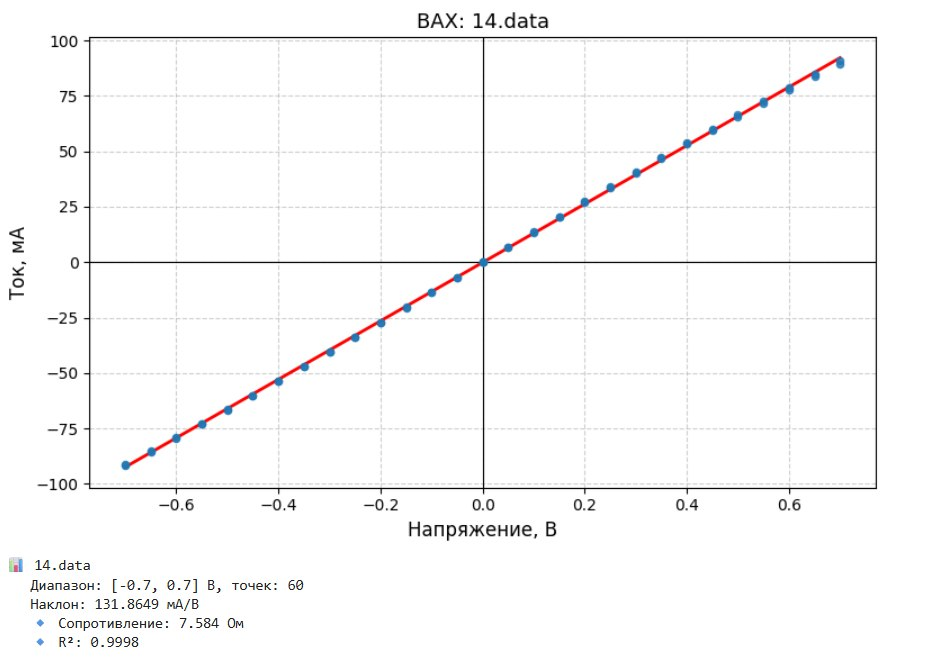
\includegraphics[width=0.75\linewidth]{d14.jpg}
    \caption{ВАХ алюминиевой рамки 1}
    \label{fig:placeholder}
\end{figure}

\begin{figure}[H]
    \centering
    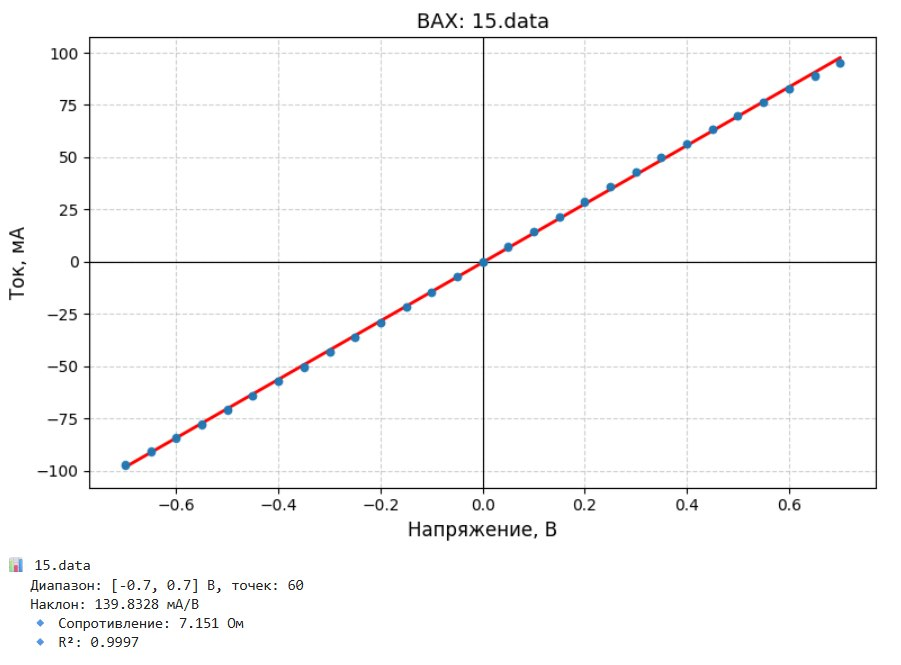
\includegraphics[width=0.75\linewidth]{d15.jpg}
    \caption{ВАХ алюминиевой рамки 2}
    \label{fig:placeholder}
\end{figure}

\subsubsection*{Измерение ВАХ между вплавленным контактом Al и рамкой}
Установим один зонд на рамку, а другой на контактную площадку вплавленного алюминия (100x100 $\text{мкм}^2$) и измерим ВАХ - она получается линейной, что говорит об оммическом контакте. По наклону определим общее сопротивление
\[
R_{\text{общee}} = 491,67\,\text{Ом}
\]

Полное сопротивление электрической схемы складывается из внутреннего сопротивления, сопротивления контактной площадки, сопротивления рамки, сопротивления кремния под контактом (сопротивление растекания):
\[
R_{\text{общее}} = R_{\text{внутреннее}} + R_{\text{рамки}} + R_{\text{Si}} + R_{\text{контакт}}
\]

Вычислим сопротивление участка рамки длиной $2$ мм, используя найденную погонную плотность:
\[
R_{\text{рамки}} = \lambda \cdot L = 0,51\,\text{Ом}
\]

Используя значение сопротивления одного контакта,
$R_{\text{контакт}} = 98.95\,\text{Ом}$ (получено в следующем пункте),
рассчитаем сопротивление растекания:
\[
R_{\text{Si}} = R_{\text{общee}} - R_{\text{внутреннее}} - R_{\text{рамки}} - R_{\text{контакт}} = 56.98\,\text{Ом}
\]
\begin{figure}[H]
    \centering
    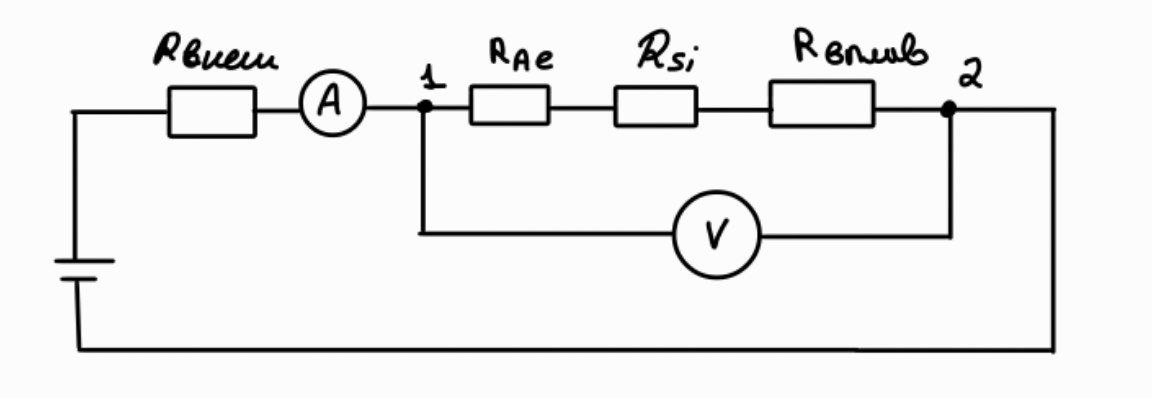
\includegraphics[width=0.75\linewidth]{image9.png}
    \caption{Электрическая схема измерения ВАХ между вплавленным контактом Al и рамкой}
    \label{fig:placeholder}
\end{figure}

\begin{figure}[H]
    \centering
    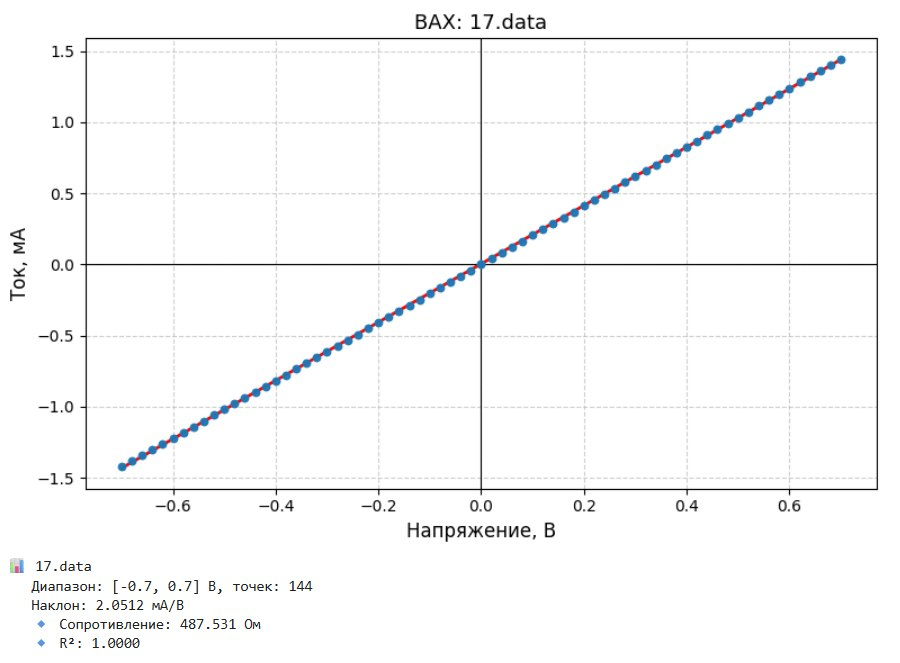
\includegraphics[width=0.75\linewidth]{d17.jpg}
    \caption{ВАХ вплавленный контакт-рамка}
    \label{fig:placeholder}
\end{figure}

\subsubsection*{Измерение ВАХ между контактными площадками вплавленного Al}
Измерим ВАХ такой структуры в двух случаях: зонды располагаются на соседних площадках и располагаются на удаленных площадках (расстояние увеличено в 7 раз). Таким образом будет найдено сопротивление контакта. Общее сопротивление складывается из сопротивления контактов, внутреннего сопротивления и сопротивления кремния между контактами:
\[
R = 2R_{\text{контакт}} + R_{\text{внутреннее}} + R_{\mathrm{Si}}
\]
Найдем сопротивление кремния между двумя соседними контактами:
\[
R_{\mathrm{Si}}
= \frac{R_{\text{удал}} - R_{\text{ближ}}}{6}
= 26,81\,\text{Ом}
\]
\[
R_{\text{ближ}} =  789,96\,\text{Ом}
\]
\[
R_{\text{удал}} =950,85\,\text{Ом}
\]
\[
R_{\text{контакт}} = \frac{R_{\text{ближ}} - R_{\text{удал}} - R_{Si}}{2}
= \frac{197.91}{2}
= 379,18\,\text{Ом}
\]

Найдем удельное сопротивление, нормированное на площадь. По порядку оно совпадает с табличным ($10^{-6} \text{ Ом}\cdot\text{м}^2$):
\[
\rho_k = R_{\text{контакт}}\cdot S
= 3,79\cdot 10^{-6}\,\text{Ом}\cdot\text{м}^2
\]
\begin{figure}[H]
    \centering
    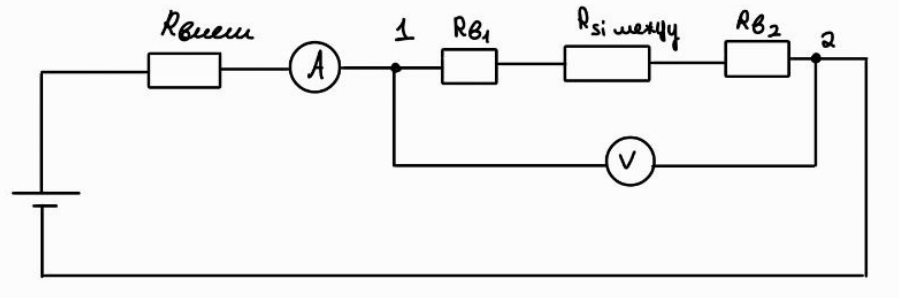
\includegraphics[width=0.65\linewidth]{image10.png}
    \caption{Электрическая схема измерения ВАХ между двумя контактными площадками вплавленного алюминия}
    \label{fig:placeholder}
\end{figure}

\begin{figure}[H]
    \centering
    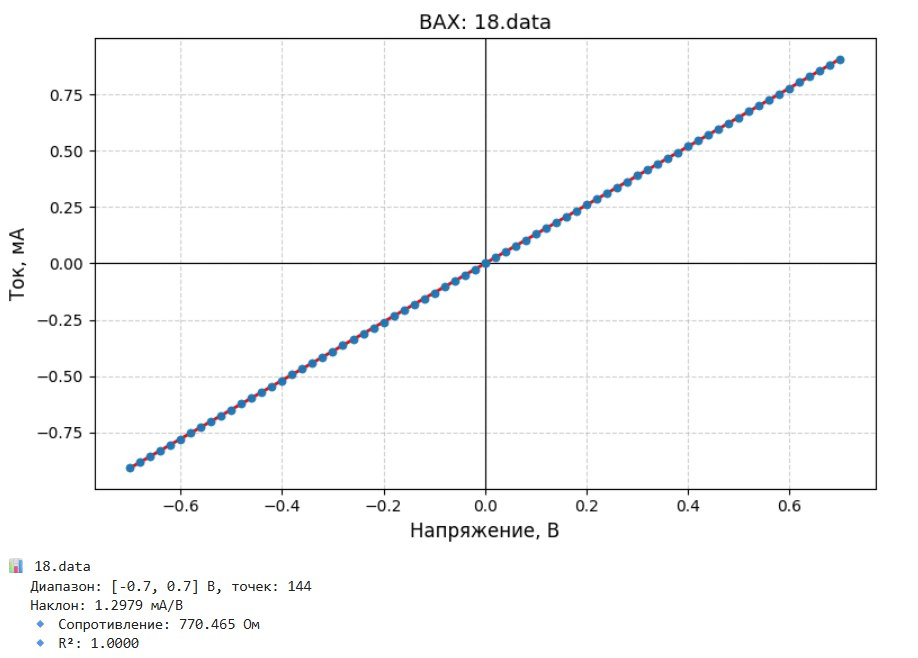
\includegraphics[width=0.75\linewidth]{d18.jpg}
    \caption{ВАХ близко расположенных контактов}
    \label{fig:placeholder}
\end{figure}

\begin{figure}[H]
    \centering
    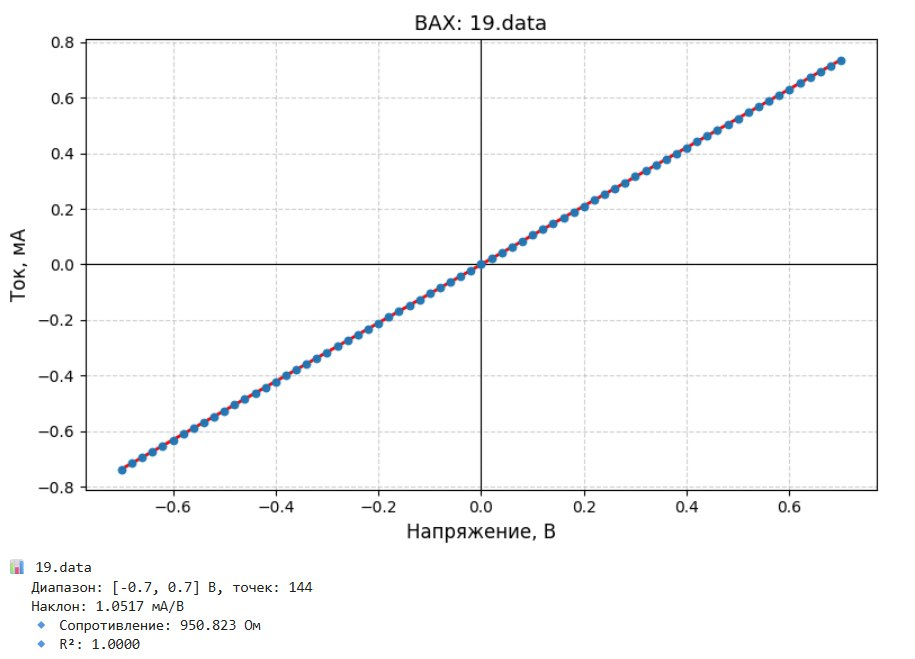
\includegraphics[width=0.75\linewidth]{d19.jpg}
    \caption{ВАХ удаленных контактов}
    \label{fig:placeholder}
\end{figure}

\subsection{Измерение параметров контакта Шоттки Al на Si}
\subsubsection*{Измерение параметров невплавленного контакта Al на Si p-типа}

Установим один зонд на алюминиевую  рамку, другой на контактную площадку невплавлен-ного алюминия, снимем ВАХ при включенном и выключенном свете.


\begin{figure}[H]
    \centering
    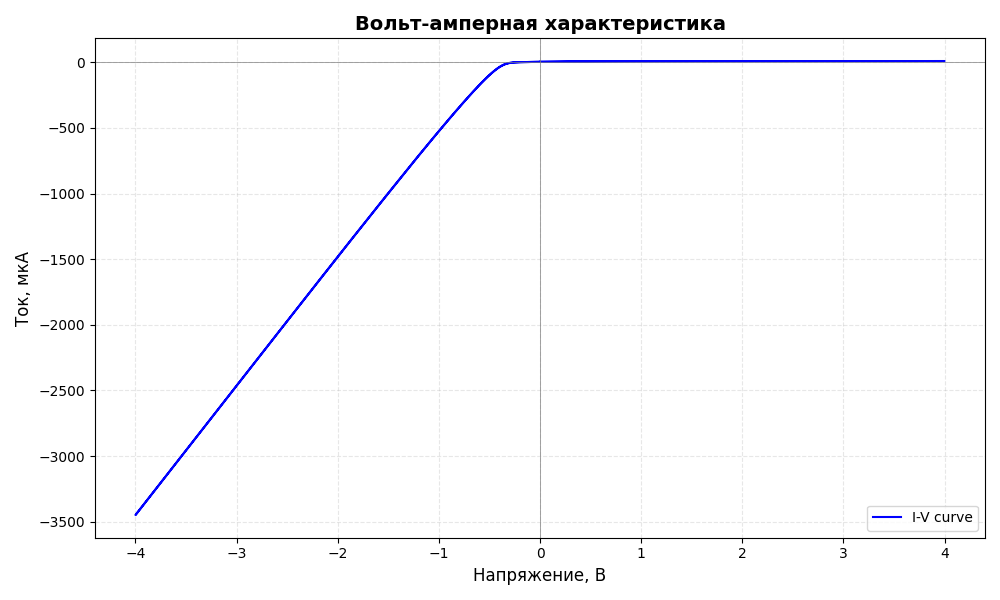
\includegraphics[width=0.85\linewidth]{F1.png}
    \caption{ВАХ при включенном свете}
    \label{fig:placeholder}
\end{figure}
% \begin{figure}[H]
%     \centering
%     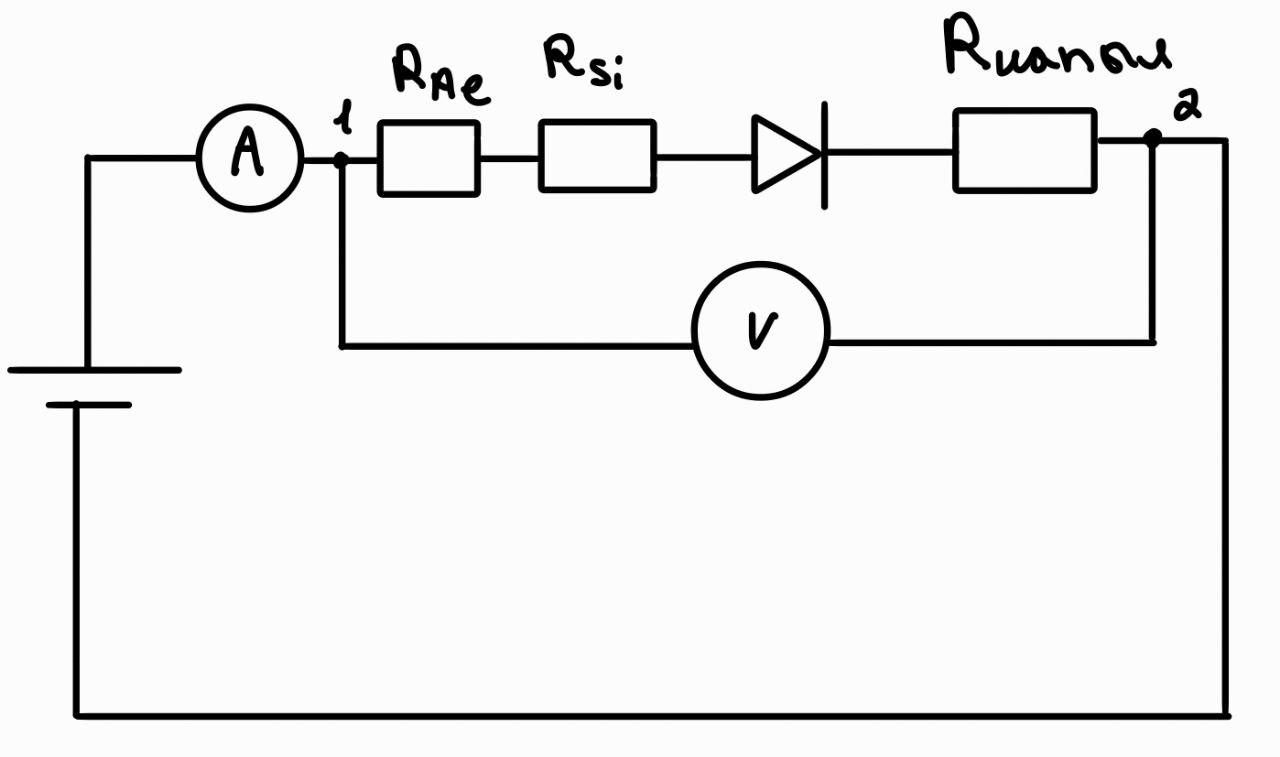
\includegraphics[width=0.5\linewidth]{image11.png}
%     \caption{Электрическая схема измерения ВАХ между двумя контактными площадками невплавленного алюминия}
%     \label{fig:placeholder}
% \end{figure}

\begin{figure}[h]
\centering
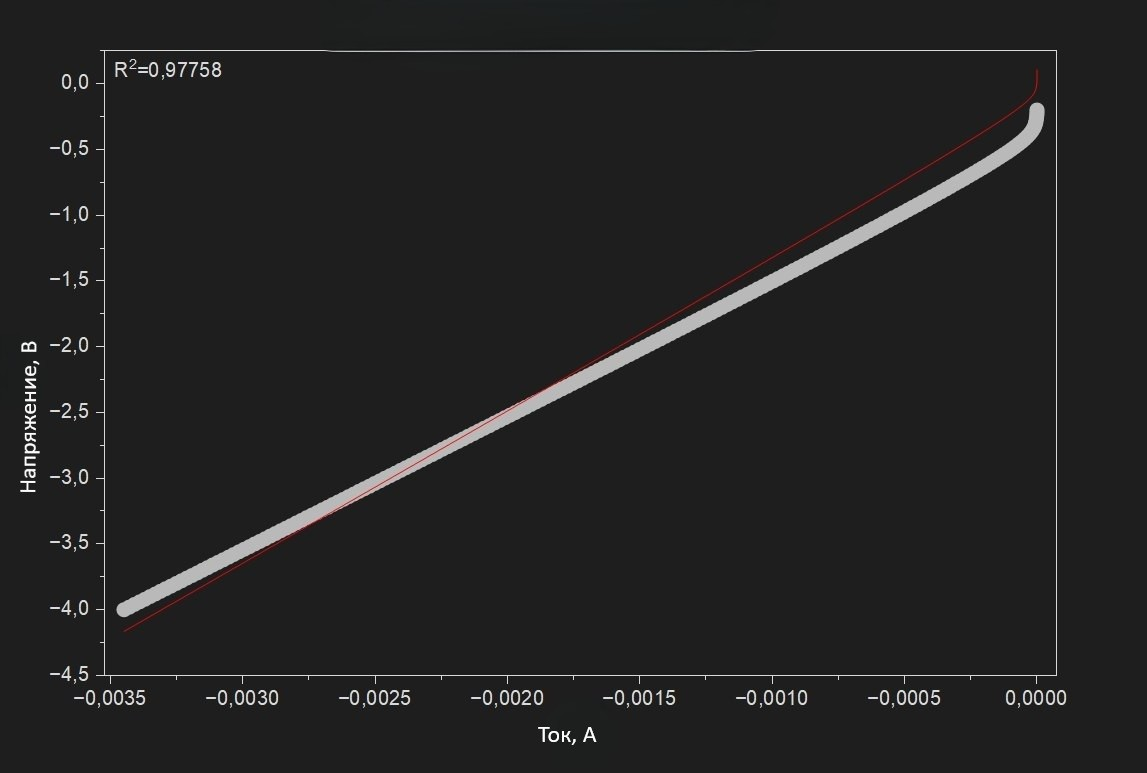
\includegraphics[width=0.9\textwidth]{p9.jpg}
\caption{Апрксимация прямой ветви ВАХ, формулой из пунукта 4.9}
\label{fig:barrier_formation}
\end{figure}

Из апрокмимации нашли I0 и R 

\begin{figure}[h]
\centering
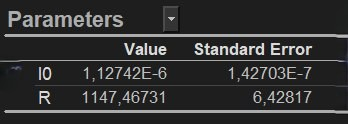
\includegraphics[width=0.9\textwidth]{pp10.jpg}
% \caption{Апрксимация прямой ветви ВАХ, формулой из пунукта 4.9}
\label{fig:barrier_formation}
\end{figure}

% По ВФХ определим: 
% \begin{enumerate}
%     \item контактную разность потенциалов  $V_\text{bi}$ по пересечению с осью напряжений
%     \item концентрацию примеси как $
% N=\frac{2}{q\,\varepsilon_s\,\varepsilon_0\,A^2\left|\dfrac{d(1/C^2)}{dV}\right|}$
%     \item емкость диода Шоттки С при нуле напряжения и экивалентного p-n перехода $
% \frac{1}{C^2}=\frac{2V_{bi}}{q\,\varepsilon_s\,\varepsilon_0\,A^2\,N}$
% \[
% C=\frac{\varepsilon_s\varepsilon_0A}{W},\quad 
% W_{\text{Ш}}=\sqrt{\frac{2\varepsilon_s\varepsilon_0(V_{bi}-V)}{qN}},\quad
% W_{p\text{-}n}=\sqrt{\frac{2\varepsilon_s\varepsilon_0(V_{bi}-V)}{q}\!\left(\frac1{N_A}+\frac1{N_D}\right)}\]

% \end{enumerate}

% \begin{figure}[H]
%     \centering
%     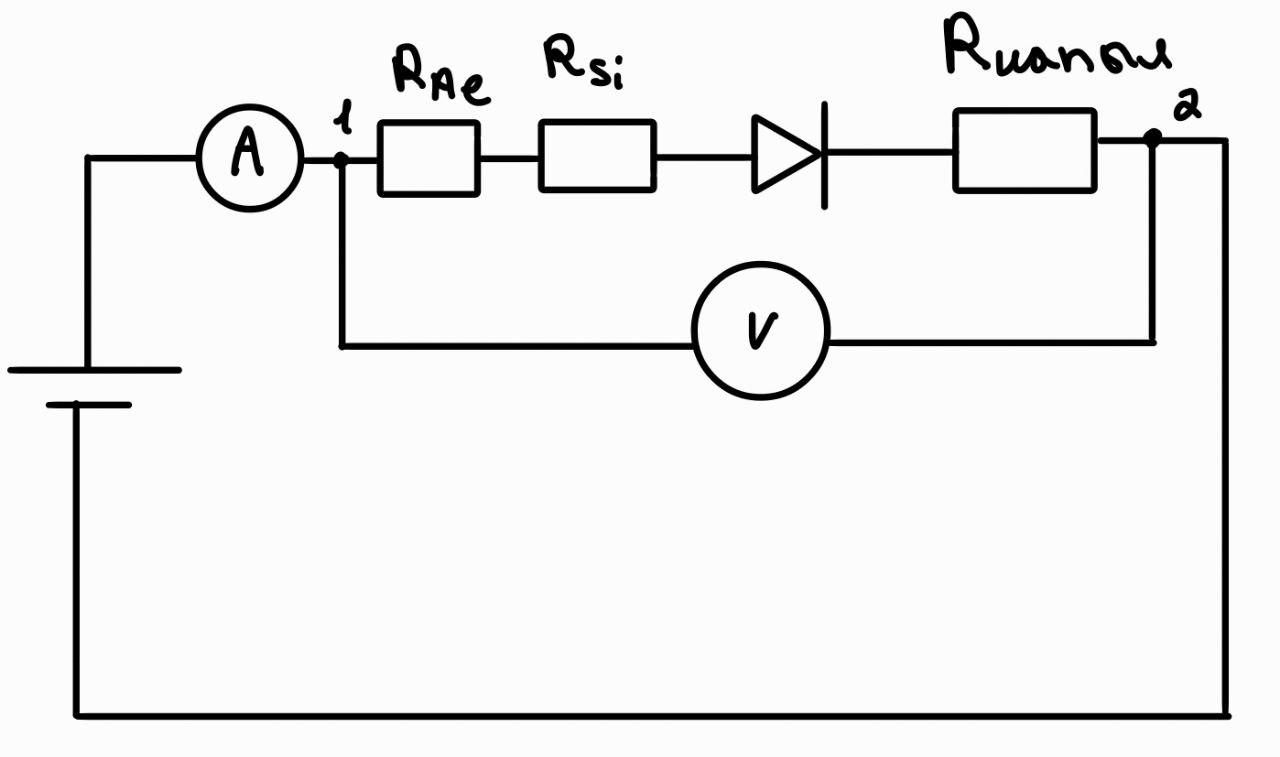
\includegraphics[width=0.5\linewidth]{image11.png}
%     \caption{Электрическая схема измерения ВАХ между двумя контактными площадками невплавленного алюминия}
%     \label{fig:placeholder}
% \end{figure}

% \begin{figure}[H]
%     \centering
%     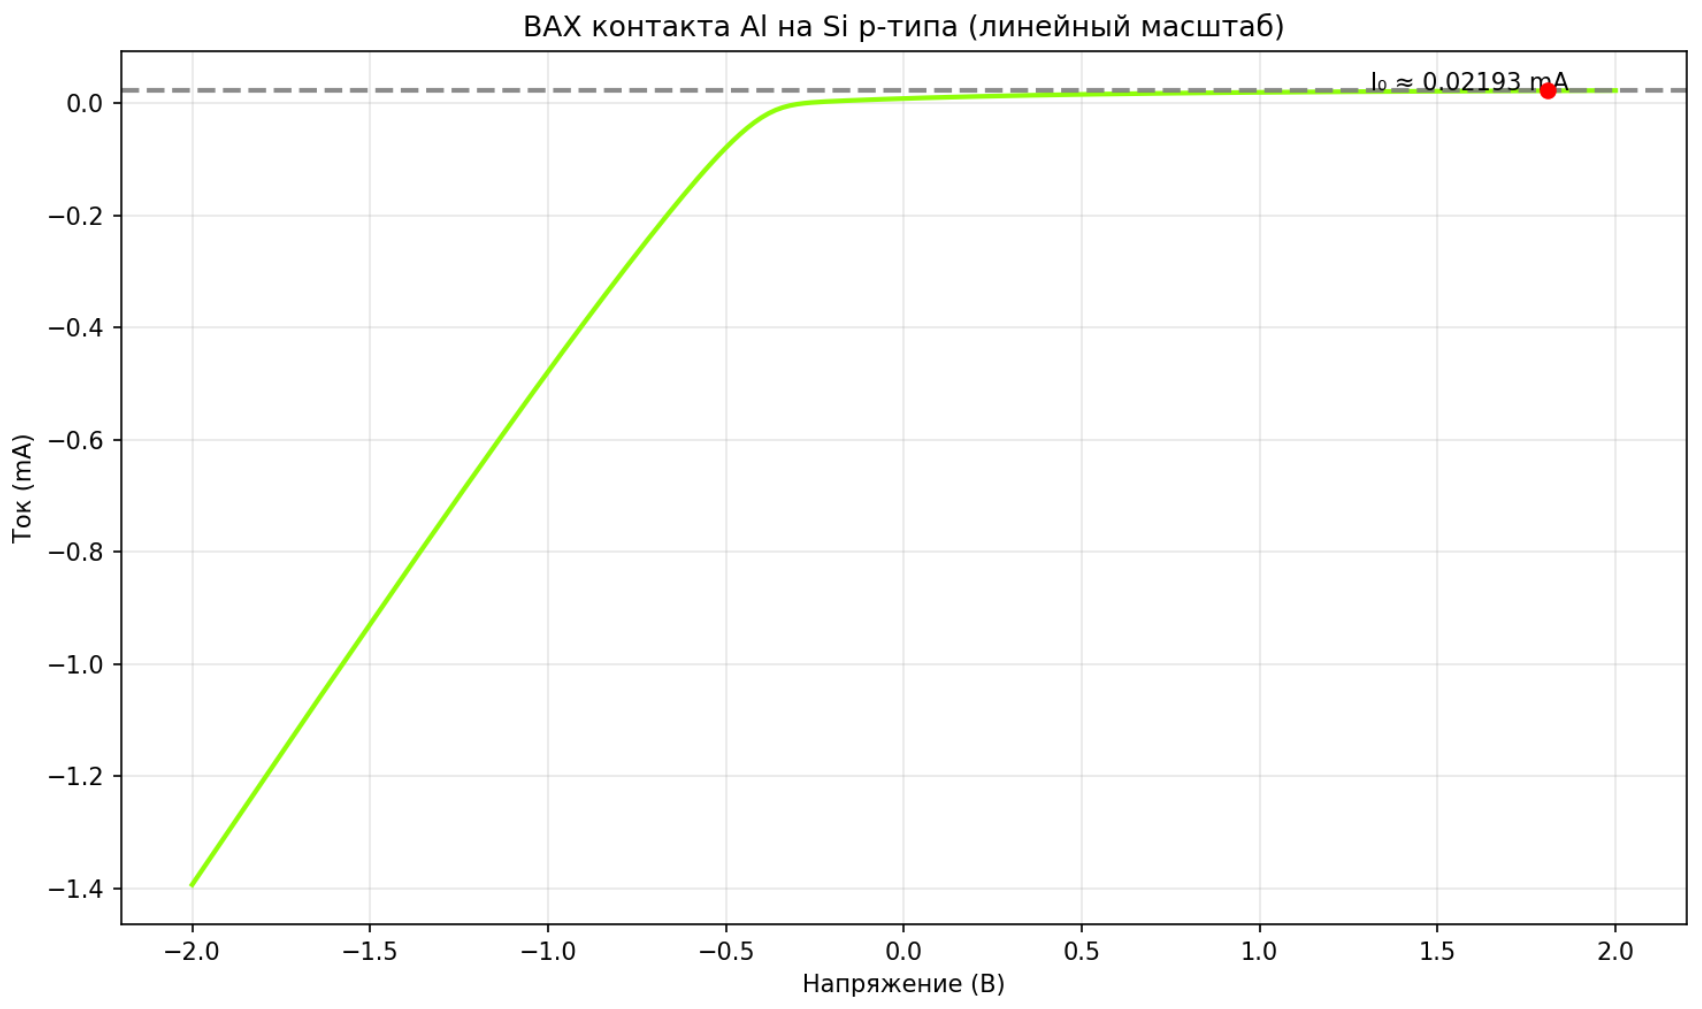
\includegraphics[width=0.85\linewidth]{image20.png}
%     \caption{ВАХ при включенном свете}
%     \label{fig:placeholder}
% \end{figure}

% \begin{figure}[H]
%     \centering
%     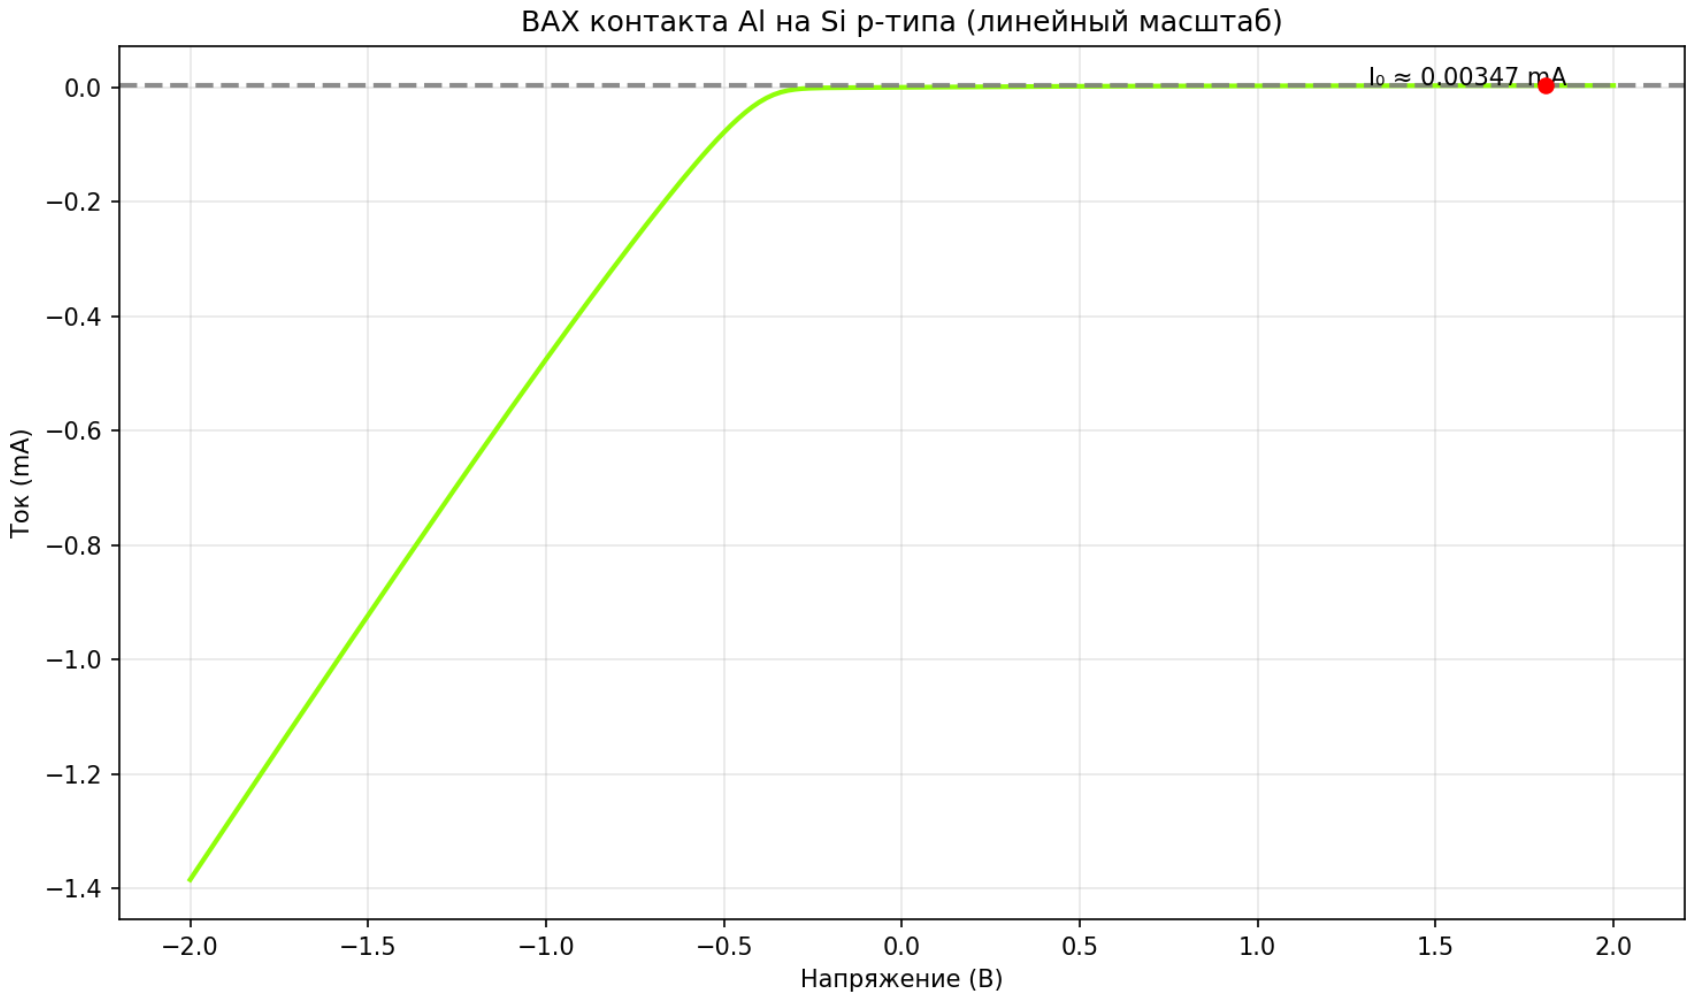
\includegraphics[width=0.85\linewidth]{image21.png}
%     \caption{ВАХ при выключенном свете}
%     \label{fig:placeholder}
% \end{figure}


% \begin{figure}[H]
%     \centering
%     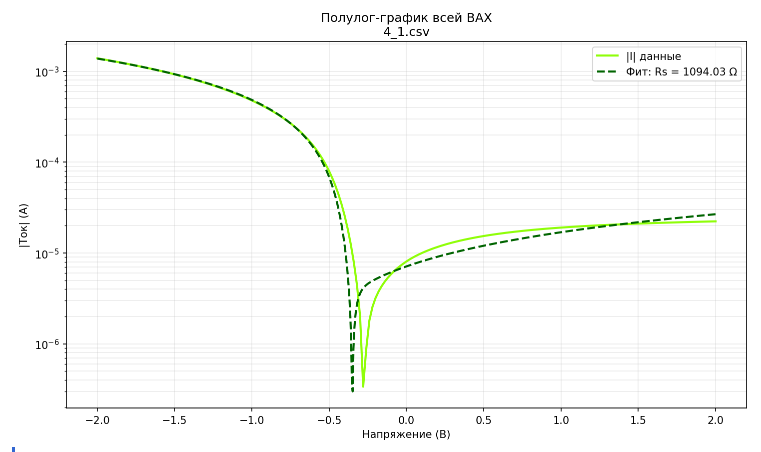
\includegraphics[width=0.85\linewidth]{image31.png}
%     \caption{Фит формулой для ВАХ диод + последовательный резистор}
%     \label{fig:placeholder}
% \end{figure}
    
% \begin{figure}[H]
%     \centering
%     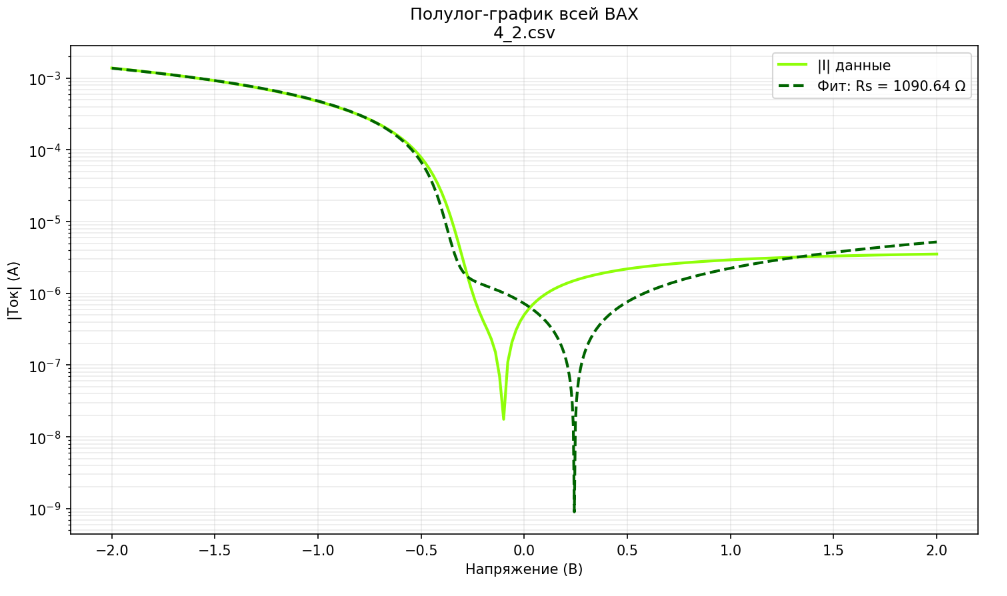
\includegraphics[width=0.85\linewidth]{image32.png}
%     \caption{Фит формулой для ВАХ диод + последовательный резистор при выключенном свете}
%     \label{fig:placeholder}
% \end{figure}
% \begin{figure}[H]
%     \centering
%     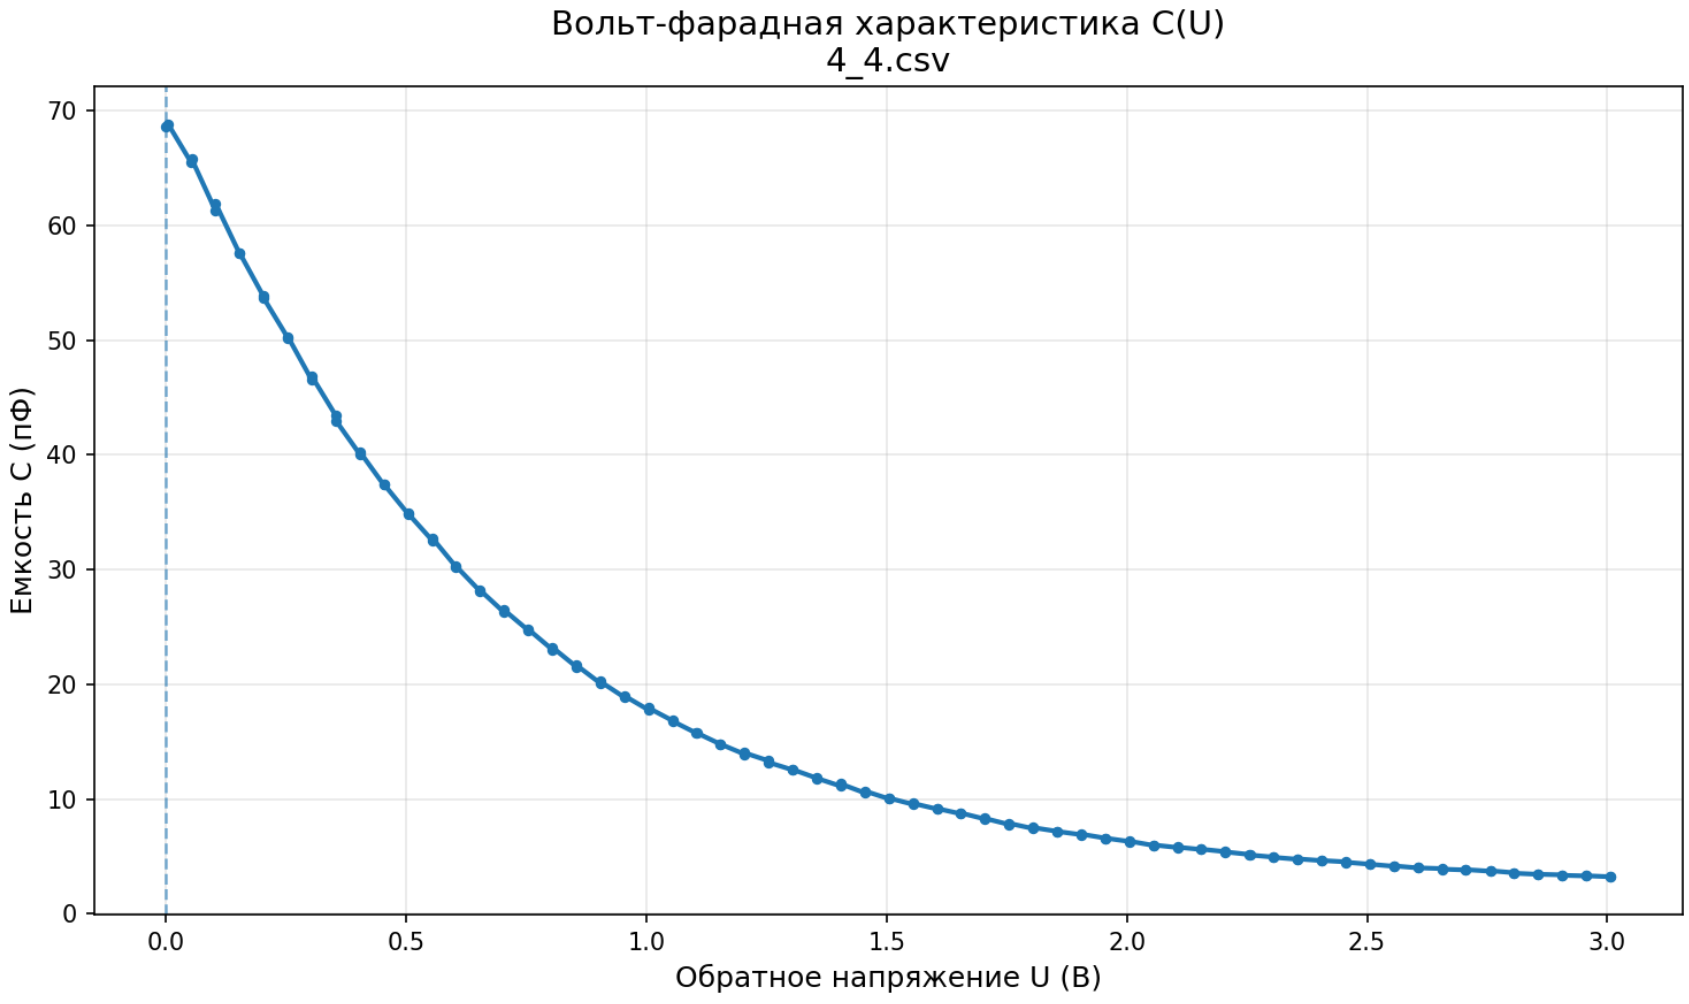
\includegraphics[width=0.85\linewidth]{image26.png}
%     \caption{ВФХ при включенном свете}
%     \label{fig:placeholder}
% \end{figure}

\begin{figure}[H]
    \centering
    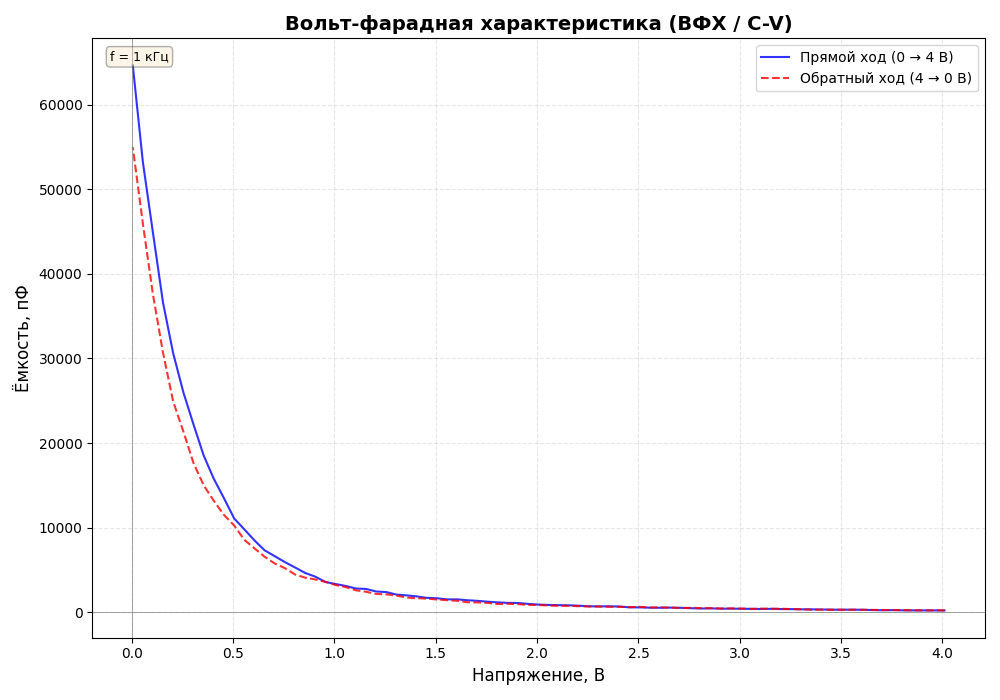
\includegraphics[width=0.7\linewidth]{F6.png}
    \caption{ВФХ при выключенном свете}
    \label{fig:placeholder}
\end{figure}

\begin{figure}[H]
    \centering
    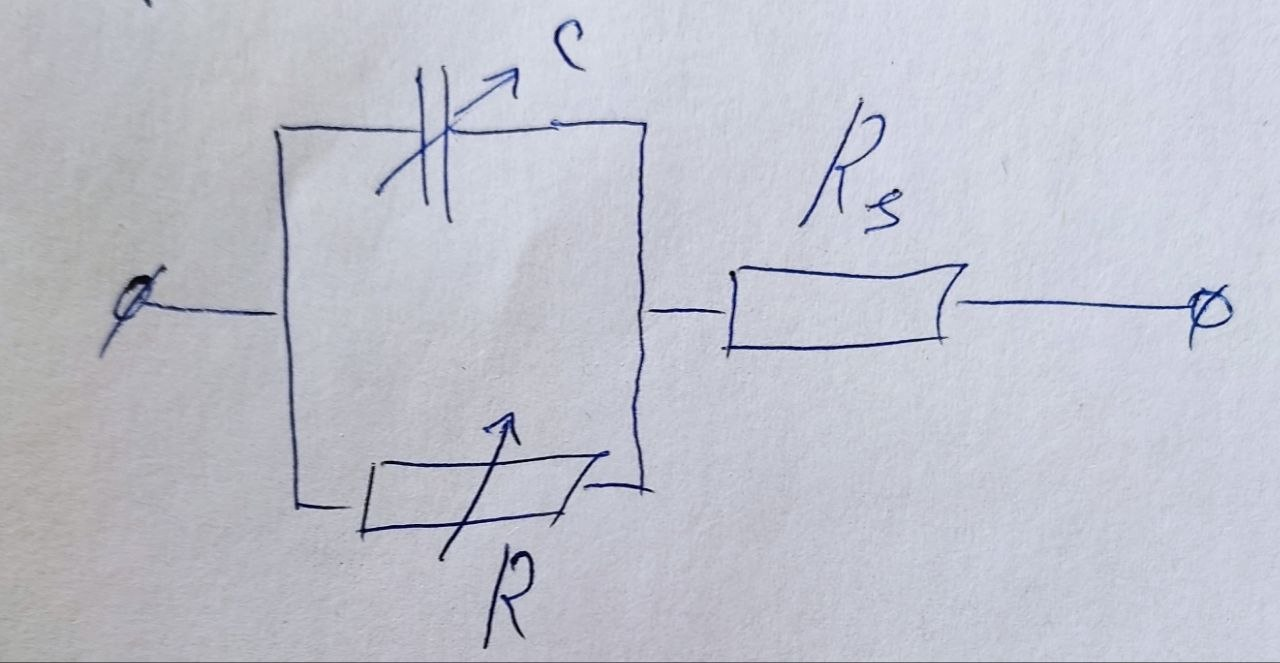
\includegraphics[width=0.7\linewidth]{pp12.jpg}
    \caption{Эквивалентая схема измерения ВФХ}
    \label{fig:placeholder}
\end{figure}

\begin{figure}[H]
    \centering
    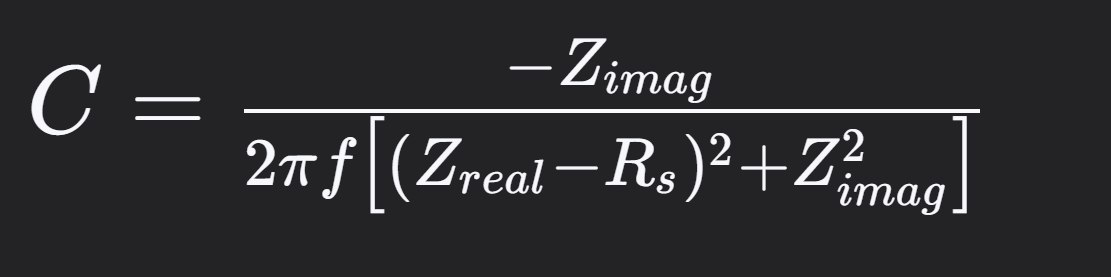
\includegraphics[width=0.7\linewidth]{pp11.jpg}
    \caption{Рабочая формула для рассчета емкости}
    \label{fig:placeholder}
\end{figure}

% \begin{figure}[H]
%     \centering
%     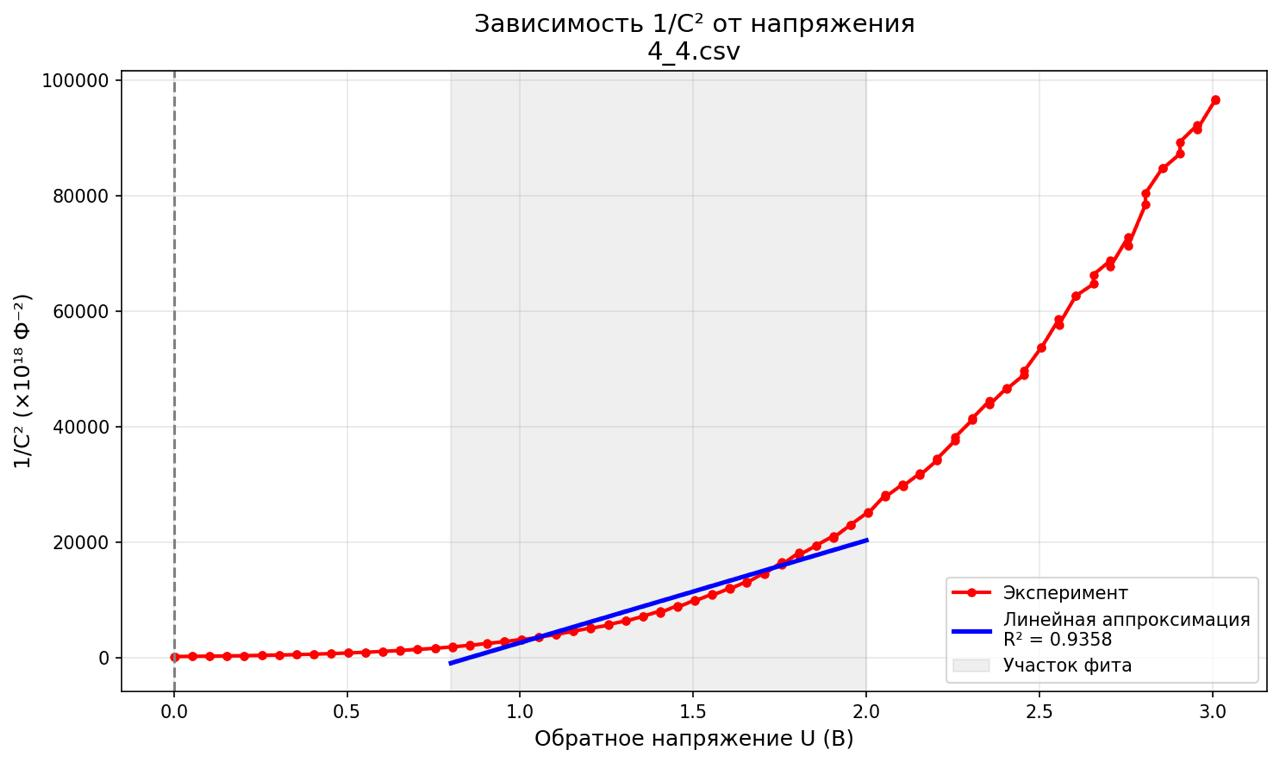
\includegraphics[width=0.85\linewidth]{image27.png}
%     \caption{$1/C^2(V)$ при включенном свете}
%     \label{fig:placeholder}
% \end{figure}

\begin{figure}[H]
    \centering
    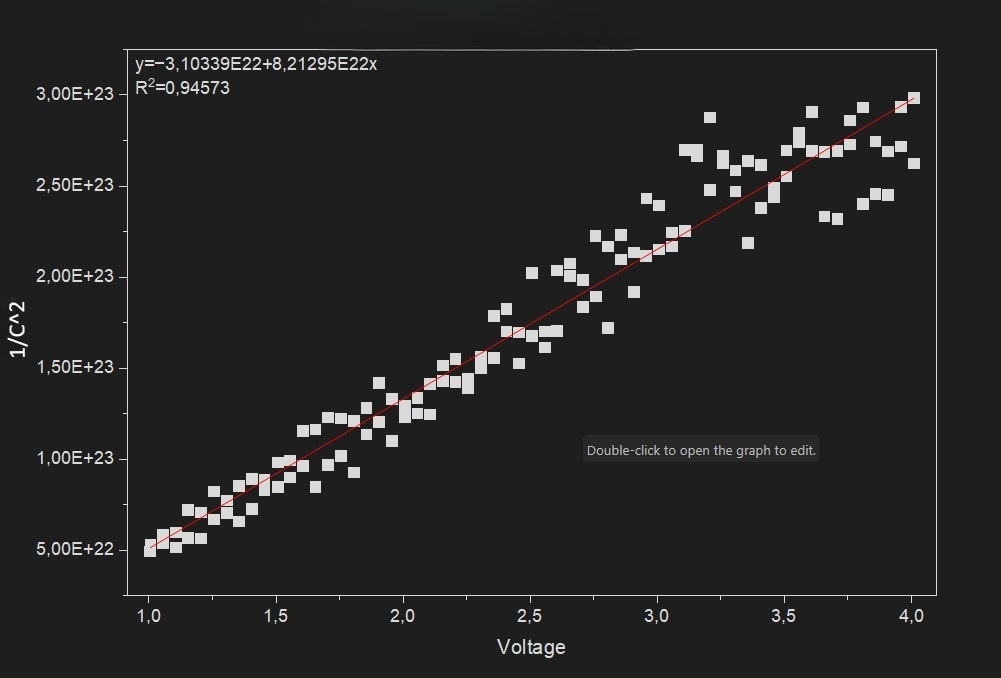
\includegraphics[width=0.7\linewidth]{pp13.jpg}
    \caption{$1/C^2(V)$}
    \label{fig:placeholder}
\end{figure}

Определим высоту энергетического барьера контакта Шоттки:

\begin{figure}[H]
    \centering
    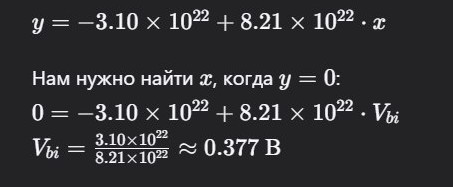
\includegraphics[width=0.85\linewidth]{pp14.jpg}
    % \caption{ВФХ при выключенном свете}
    \label{fig:placeholder}
\end{figure}

Используя эти данные вычислим концентрацию лигирующих примесей:

\begin{figure}[H]
    \centering
    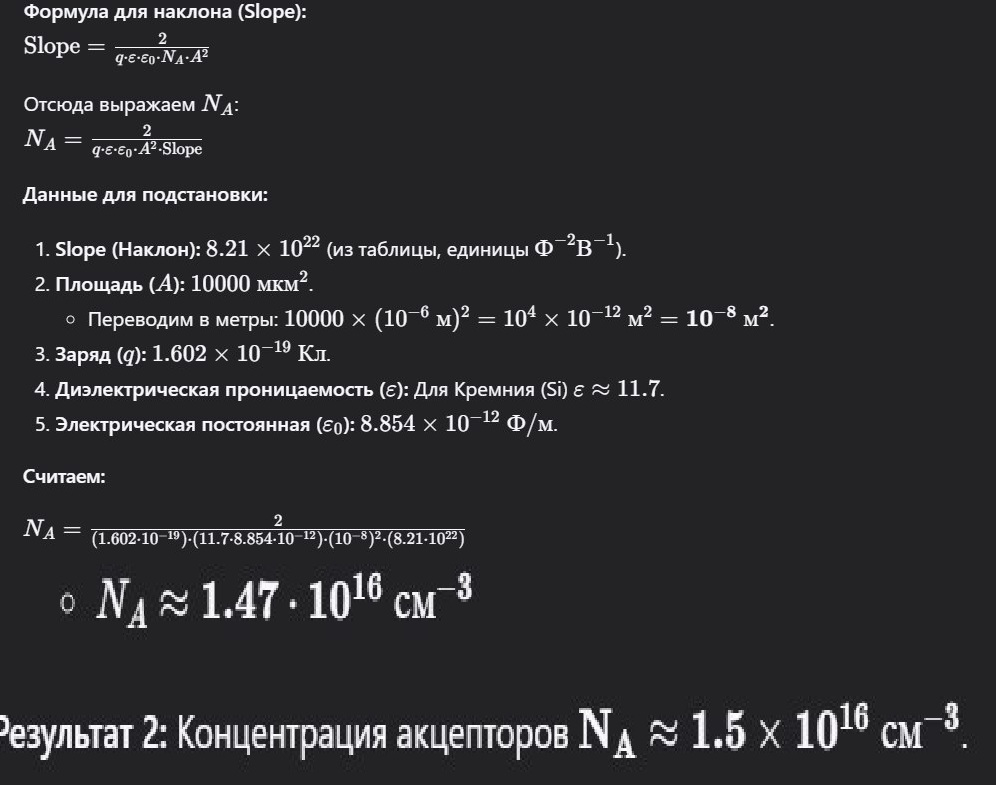
\includegraphics[width=0.85\linewidth]{pp15.jpg}
    % \caption{ВФХ при выключенном свете}
    \label{fig:placeholder}
\end{figure}

\subsubsection*{Измерения для невплавленных контактов}
Установим один зонд на невплавленный контакт алюминия, другой на контактную площадку тоже невплавленного алюминия, снимем ВАХ и ВФХ при выключенном свете.

%     \item емкость диода Шоттки С при нуле напряжения и экивалентного p-n перехода $
% \frac{1}{C^2}=\frac{2V_{bi}}{q\,\varepsilon_s\,\varepsilon_0\,A^2\,N}$
% \[
% C=\frac{\varepsilon_s\varepsilon_0A}{W},\quad 
% W_{\text{Ш}}=\sqrt{\frac{2\varepsilon_s\varepsilon_0(V_{bi}-V)}{qN}},\quad
% W_{p\text{-}n}=\sqrt{\frac{2\varepsilon_s\varepsilon_0(V_{bi}-V)}{q}\!\left(\frac1{N_A}+\frac1{N_D}\right)}\]

% \[\xrightarrow{\,N_A=N_D=N\,}\sqrt2\,W_{\text{Ш}}
% \Rightarrow C_{p\text{-}n}(0)=\frac{C_{\text{Ш}}(0)}{\sqrt2}.
% \]


% \begin{figure}[H]
%     \centering
%     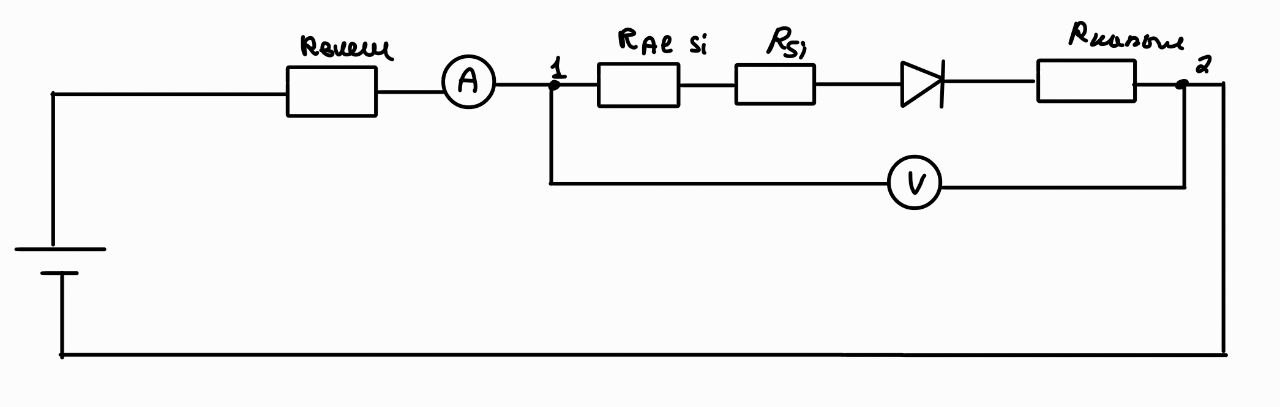
\includegraphics[width=0.75\linewidth]{image12.png}
%     \caption{Электрическая схема измерения ВАХ между вплавленным и напыленным контактами Al}
%     \label{fig:placeholder}
% \end{figure}

\begin{figure}[H]
    \centering
    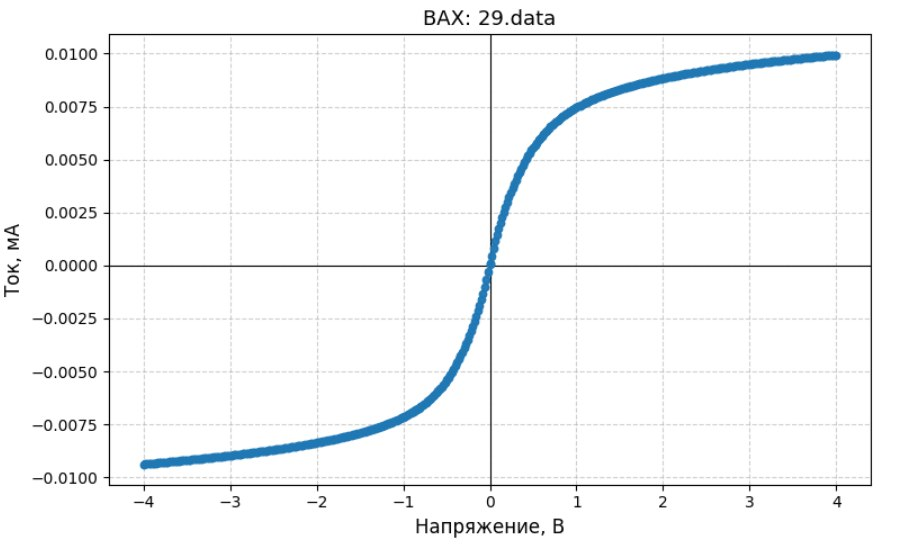
\includegraphics[width=0.85\linewidth]{p71.jpg}
    \caption{ВАХ для выключенного света}
    \label{fig:placeholder}
\end{figure}

% \begin{figure}[H]
%     \centering
%     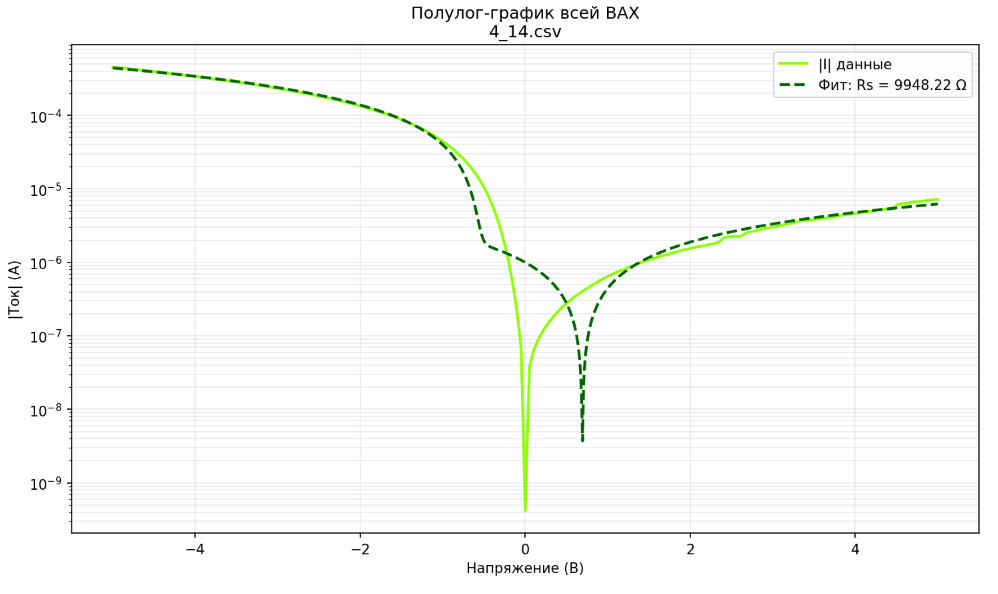
\includegraphics[width=0.85\linewidth]{image33.png}
%     \caption{Фит формулой для ВАХ диод + последовательный резистор}
%     \label{fig:placeholder}
% \end{figure}

\begin{figure}[H]
    \centering
    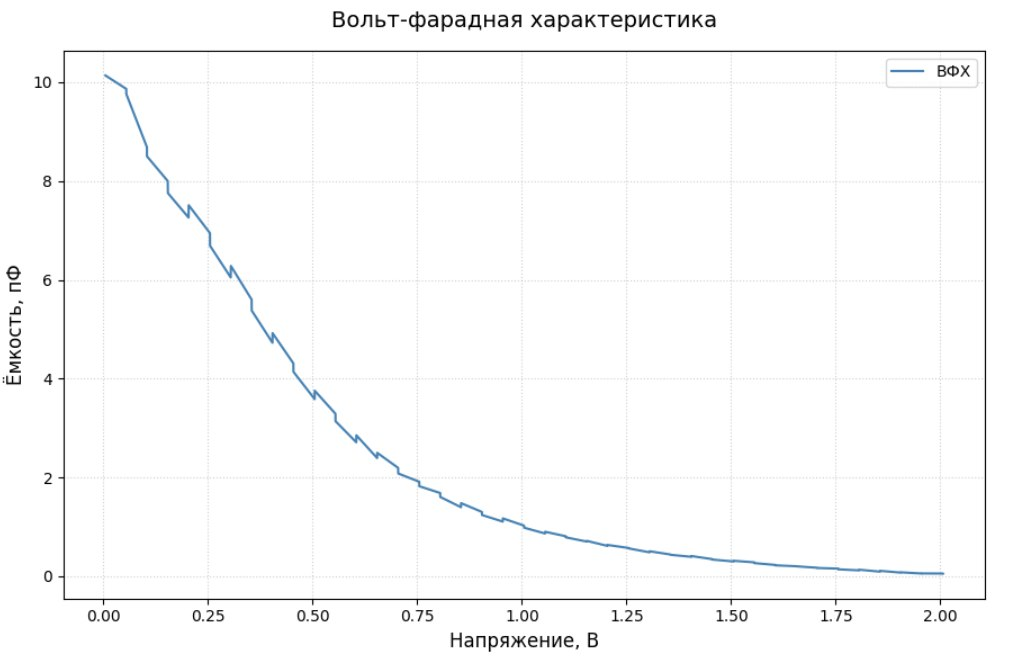
\includegraphics[width=0.85\linewidth]{p73.jpg}
    \caption{ВФХ при выключенном свете}
    \label{fig:placeholder}
\end{figure}

\subsection{Выводы и полученные результаты}


% \begin{table}[H]
% \centering
% \begin{tabular}{|c|c|c|c|}
% \hline
%  & Рамка-напыление, свет есть & Рамка-напыление, света нет & Вплавл-напыл, света нет \\
% \hline

% $I_0$, A 
% & $2.19 \cdot 10^{-5}$ 
% & $0.35 \cdot 10^{-5}$ 
% & $0.61 \cdot 10^{-5}$ \\
% \hline

% $\eta$ 
% & 1.31 
% & 1.78 
% & 4.74 \\
% \hline

% $\varphi_s$, эВ 
% & 0.457 
% & 0.505 
% & 0.480 \\
% \hline

% \end{tabular}
% \caption{Параметры диода Шоттки, определенные из ВАХ диода}
% \end{table}


% \begin{table}[H]
% \centering
% \begin{tabular}{ccccccccc}
% \toprule
% Файл &
% $\frac{d(1/C^2)}{dV}$, Ф$^{-2}$/В &
% $R^2$ &
% $V_{bi}$, В &
% $N_A$, м$^{-3}$ &
% $N_A$, см$^{-3}$ &
% $C_{\text{Ш}}(0)$, пФ &
% $C_{p\text{-}n}(0)$, пФ \\
% \midrule
% 1 &
% $1.77\cdot10^{22}$ &
% 0.936 &
% 0.853 &
% $6.80\cdot10^{22}$ &
% $6.80\cdot10^{16}$ &
% 9.42 &
% 6.66 \\

% 2 &
% $1.78\cdot10^{22}$ &
% 0.93 &
% 0.85 &
% $6.77\cdot10^{22}$ &
% $6.77\cdot10^{16}$ &
% 9.39 &
% 6.64 \\

% 3 &
% $8.81\cdot10^{21}$ &
% 0.906 &
% 0.947 &
% $1.37\cdot10^{23}$ &
% $1.367\cdot10^{17}$ &
% 11.81 &
% 8.35 \\
% \bottomrule
% \end{tabular}
% \caption{Параметры барьера Шоттки, определённые из линейной аппроксимации зависимости $1/C^2(U)$}
% \end{table}

\section*{Выводы}

В ходе выполнения лабораторной работы были исследованы вольт-амперная (ВАХ) и вольт-фарадная (ВФХ) характеристики диода Шоттки на основе кремния (p-тип, площадь контакта $A = 10^4$~мкм$^2$).

\begin{enumerate}
    \item \textbf{Анализ ВАХ.} 
    Экспериментальная зависимость тока от напряжения была аппроксимирована уравнением диода с учётом последовательного сопротивления:
    \begin{equation}
        I = I_0 \left[ \exp\left(\frac{q(U - I R_s)}{k T}\right) - 1 \right].
    \end{equation}
    Методом нелинейной регрессии (Levenberg-Marquardt) были определены параметры:
    \begin{itemize}
        \item Ток насыщения: $I_0 = 1,12 \pm 0.14 \times 10^{-6}$ А;
        \item Последовательное сопротивление: $R_s = (1147 \pm 15)$~Ом.
    \end{itemize}
    Коэффициент детерминации $R^2 = 0.977$ свидетельствует о хорошем согласии модели с экспериментом.

    \item \textbf{Анализ ВФХ и график Мотта-Шоттки.}
    На основе измеренного импеданса была рассчитана барьерная ёмкость перехода $C(U)$ с учётом найденного ранее $R_s$. Построена зависимость $1/C^2$ от напряжения $U$ (график Мотта-Шоттки) в области обратного смещения.
    
    Линейная аппроксимация участка $1.5\text{--}3.0$~В дала уравнение:
    \begin{equation}
        \frac{1}{C^2} = (-3.10 \times 10^{22}) + (8.21 \times 10^{22}) \cdot U, \quad R^2 = 0.94.
    \end{equation}

    \item \textbf{Определение физических параметров.}
    Из параметров линейного фита были рассчитаны:
    \begin{itemize}
        \item Встроенный потенциал (контактная разность потенциалов):
        \begin{equation}
            V_{bi} \approx 0.38~\text{В}.
        \end{equation}
        \item Концентрация акцепторов в полупроводнике ($\varepsilon_{Si} = 11.7$):
        \begin{equation}
            N_A = \frac{2}{q \varepsilon \varepsilon_0 A^2 \cdot \text{Slope}} \approx 1.5 \times 10^{16}~\text{см}^{-3}.
        \end{equation}
    \end{itemize}
\end{enumerate}

\noindent \textbf{Заключение:} Полученные значения $V_{bi}$ и $N_A$ находятся в диапазоне, характерном для контактов металл--полупроводник на кремниевых подложках, что подтверждает корректность проведённых измерений и обработки данных.


% Попробуем построить ВФХ при учтенном сопротивлении: параллельном и последовательно соединенным.По ним определим новые емкости и концентрации

% \begin{figure}[H]
%     \centering
%     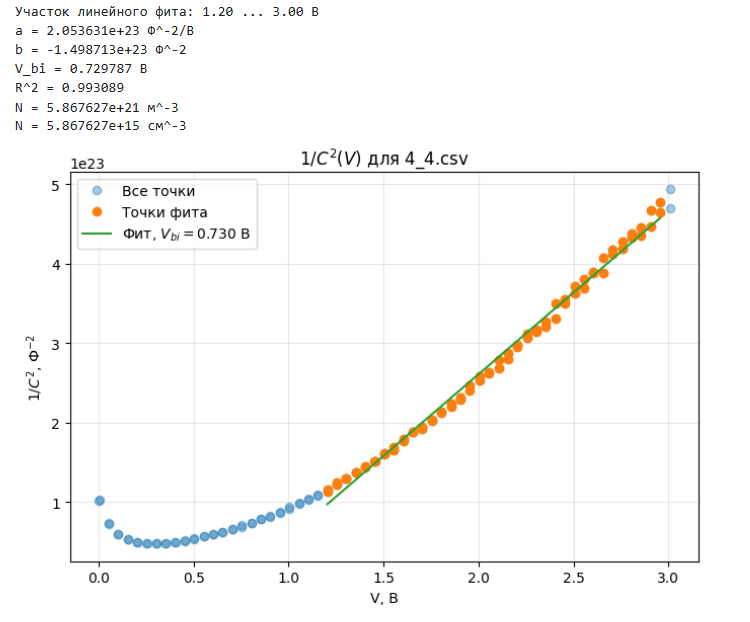
\includegraphics[width=0.75\linewidth]{image34.png}
%     \caption{$1/C^2(V)$ для первого случая}
%     \label{fig:placeholder}
% \end{figure}

% \begin{figure}[H]
%     \centering
%     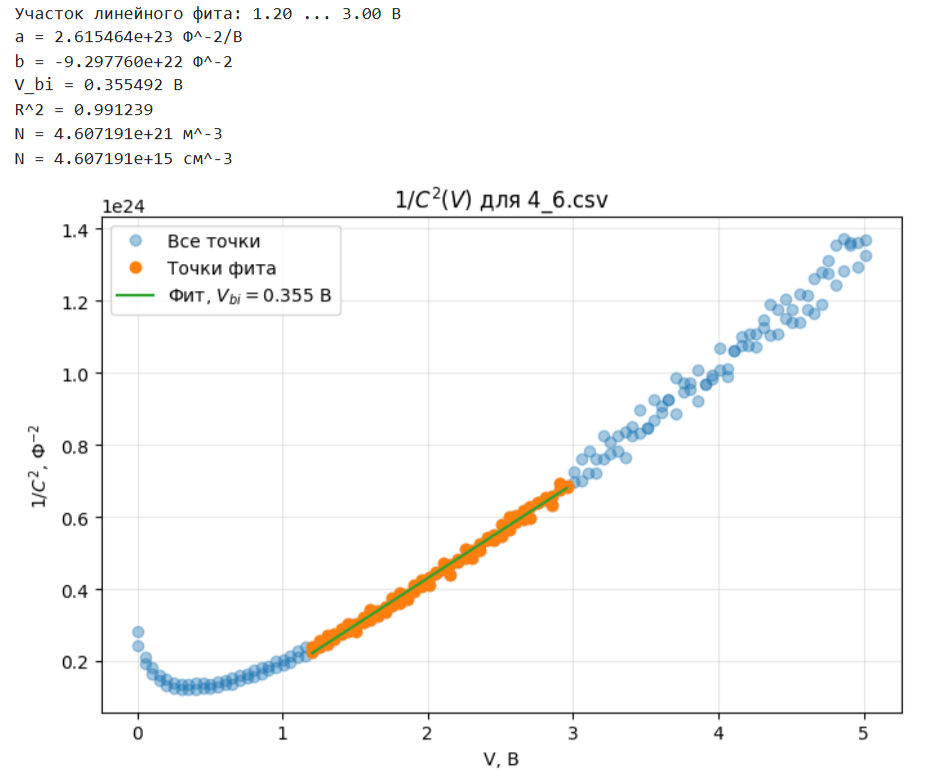
\includegraphics[width=0.75\linewidth]{image36.png}
%     \caption{$1/C^2(V)$ для второго случая}
%     \label{fig:placeholder}
% \end{figure}

% \begin{figure}[H]
%     \centering
%     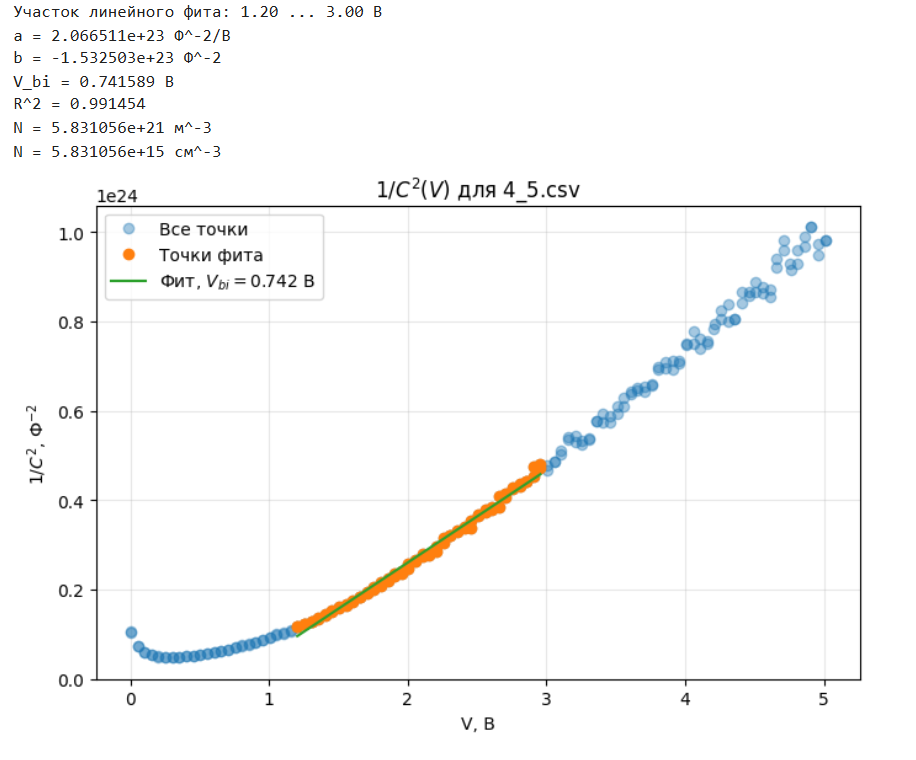
\includegraphics[width=0.75\linewidth]{image35.png}
%     \caption{$1/C^2(V)$ для третьего случая}
%     \label{fig:placeholder}
% \end{figure}

% \begin{figure}[H]
%     \centering
%     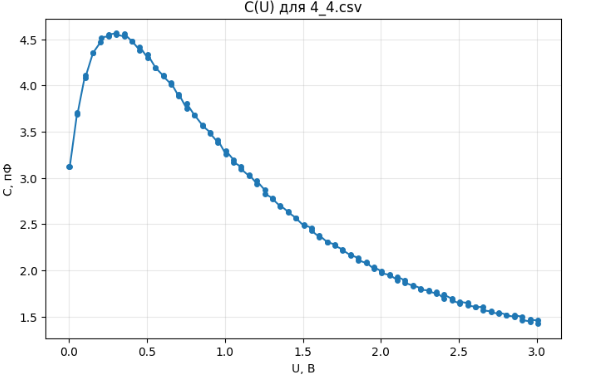
\includegraphics[width=0.75\linewidth]{image37.png}
%     \caption{ВФХ для первого случая}
%     \label{fig:placeholder}
% \end{figure}
% \begin{figure}[H]
%     \centering
%     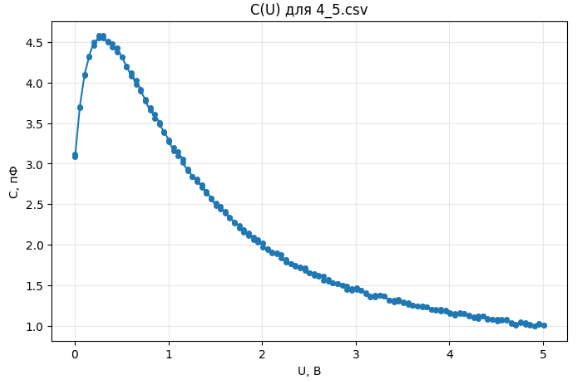
\includegraphics[width=0.75\linewidth]{image38.png}
%     \caption{ВФХ для второго случая}
%     \label{fig:placeholder}
% \end{figure}
% \begin{figure}[H]
%     \centering
%     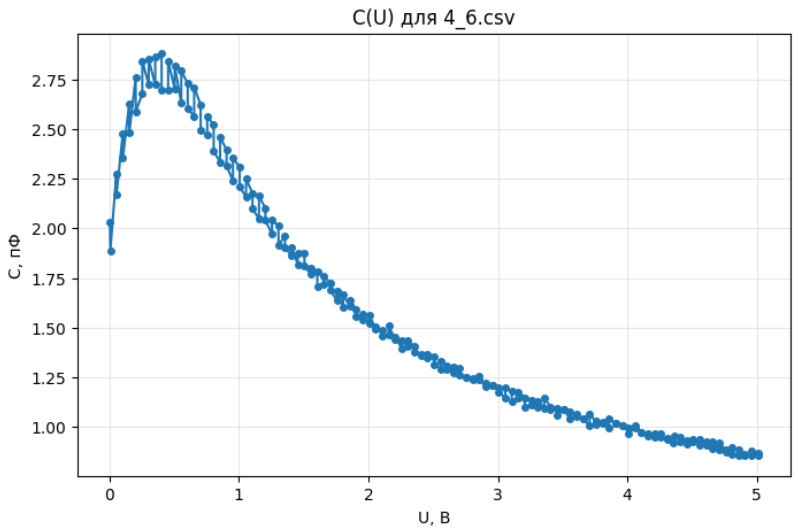
\includegraphics[width=0.75\linewidth]{image39.png}
%     \caption{ВФХ для третьего случая}
%     \label{fig:placeholder}
% \end{figure}

% \begin{figure}[H]
%     \centering
%     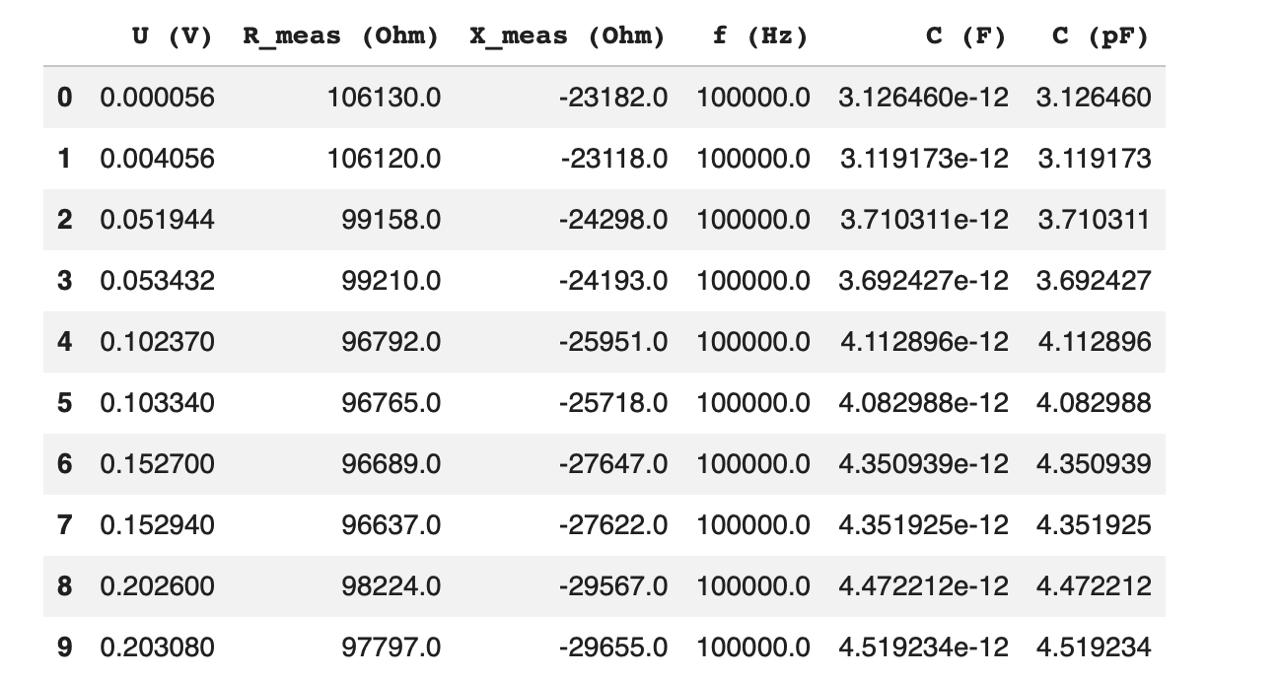
\includegraphics[width=0.75\linewidth]{image40.png}
%     \caption{Данные с ВФХ 1}
%     \label{fig:placeholder}
% \end{figure}

% \begin{figure}[H]
%     \centering
%     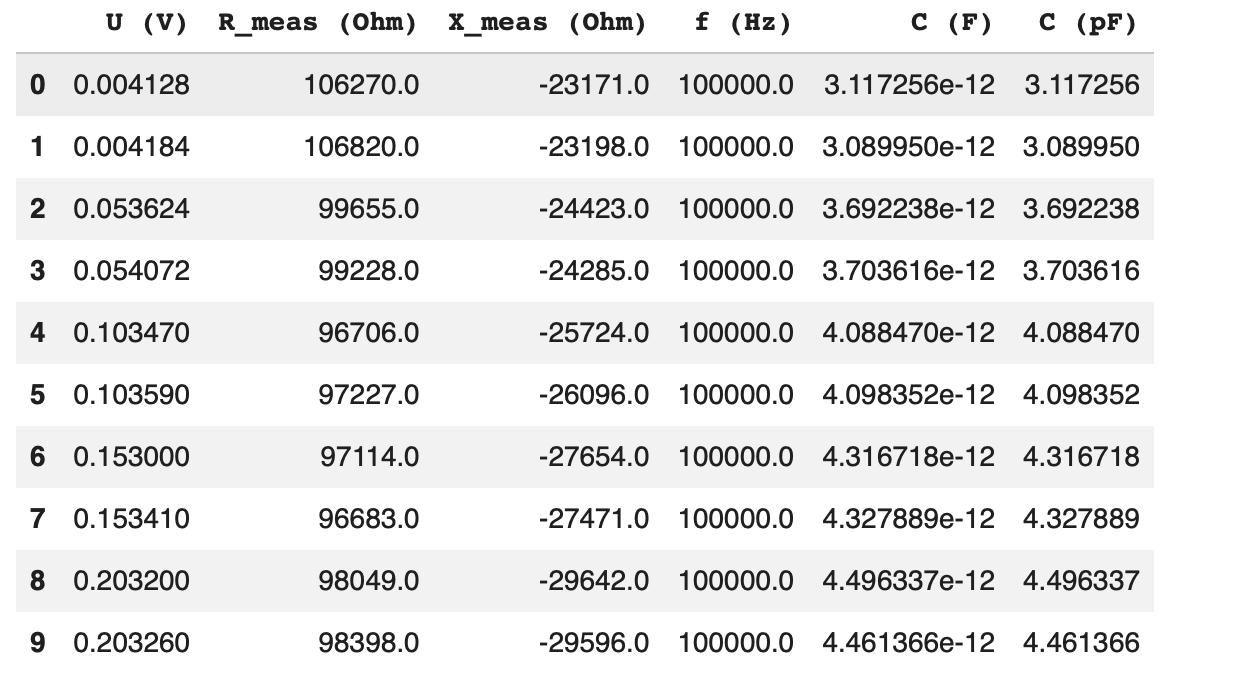
\includegraphics[width=0.75\linewidth]{image41.png}
%     \caption{Данные с ВФХ 2}
%     \label{fig:placeholder}
% \end{figure}

% \begin{figure}[H]
%     \centering
%     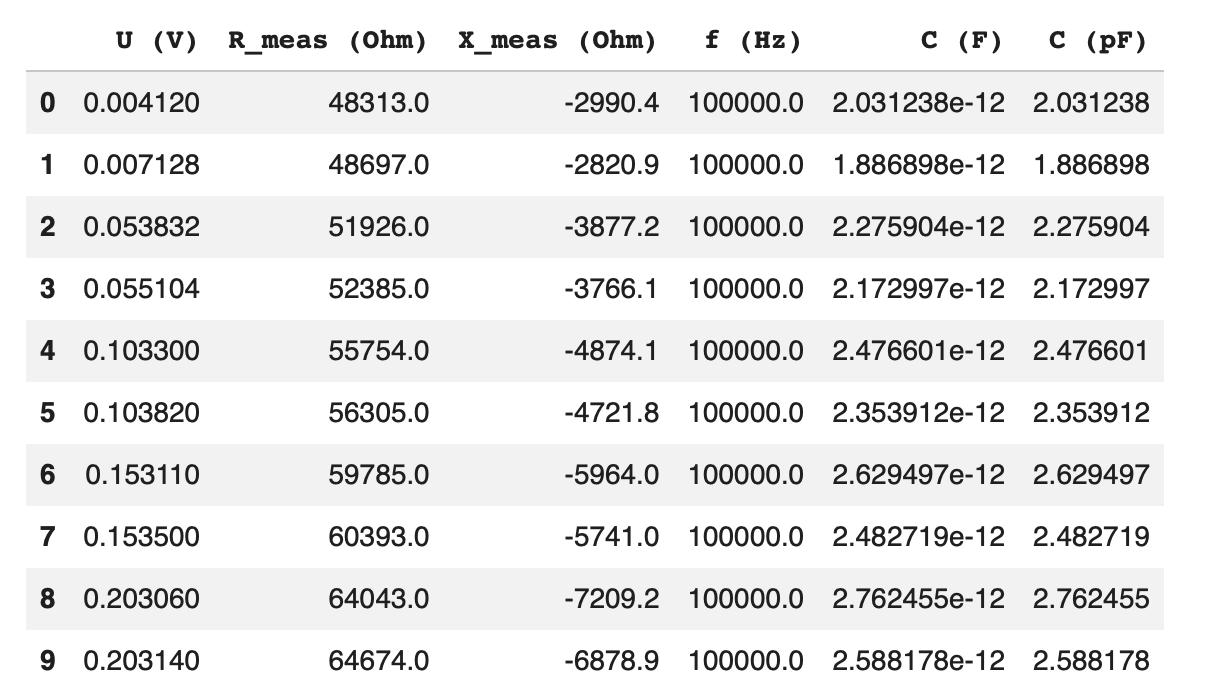
\includegraphics[width=0.75\linewidth]{image42.png}
%     \caption{Данные с ВФХ 3}
%     \label{fig:placeholder}
% \end{figure}
\end{document}